\documentclass[11pt]{article}

\usepackage{graphicx}
\usepackage[dvipsnames]{color}
\usepackage[hidelinks]{hyperref}
\usepackage[numbers]{natbib}
%pPara poder modificar los margenes
\usepackage{vmargin}
%Para usar el español
\usepackage[spanish]{babel}
\usepackage[utf8]{inputenc}

\begin{document}
%Portada
\setpapersize{A4}
\begin{titlepage}
	\centering
	{
\includegraphics[width=0.8\textwidth]{logo}\par}
	\vspace{1cm}
	{\Large Facultad de Ingeniería Informática \par}
	\vspace{3cm}
	{\scshape\Huge Aplicación web de soporte al Aprendizaje-Servicio \par}
	\vspace{5cm}
	{\textbf\Large Autores \par}
	{\Large Daniela-Nicoleta Boldureanu (Grado en Ingeniería del Software)\par}
	{\Large Victoria Gnatiuk Romaniuk (Grado en Ingeniería Informática)\par}
	{\Large Jesús Sánchez Granado (Grado en Ingeniería Informática\par}
	\vspace{1cm}
	{\textbf\Large Tutores \par}
	{\Large Simon Pickin \par}
	{\Large Manuel Montenegro Montes \par}
	
\end{titlepage}

%Indice
\tableofcontents
\newpage
\listoffigures
\section{Contexto de la propuesta}
\subsection{Introducción}
El aprendizaje-servicio es una propuesta educativa que combina aprendizaje y servicios a la comunidad.  Estos proyectos permiten a los alumnos aprender de una forma más práctica, aplicando sus conocimientos adquiridos en clase mediante la realización de tareas útiles para la comunidad. \\\\
Además de darles la oportunidad de aplicar sus conocimientos en un entorno real, les impulsa a comprender el funcionamiento de la sociedad y las responsabilidades sociales que estos tienen por forma parte de una sociedad.\\\\
Todo proyecto ApS empieza por una iniciativa con una necesidad social real que implica la ejecución de un servicio para solventarla y tiene como objetivo el aprendizaje y la reflexión del alumno.
\subsection{Elementos que intervienen en un proyecto ApS}
\begin{itemize} 
	\item El alumno es el individuo que aplica sus conocimientos teóricos en un entorno físico beneficiando a su comunidad. Además de adquirir habilidades prácticas relacionadas con su formación es importante que se incite al alumno a reflexionar sobre sus actos y el impacto positivo que tienen estos sobre los demás. Esto permite al alumno adquirir compromiso social y desarrollar pensamiento ético, cultivando un ciudadano responsable capaz de mejorar la sociedad de la que forma parte.
	\item El profesor es el individuo que se encarga de guiar al alumno en todo el proceso del proyecto, evaluando sus tareas e incitando al alumno a la reflexión. Además de guiar al alumno en su formación y gestionar el proyecto, ofrece su formación y conocimientos a la entidad. El profesor se encarga de acordar y organizar los proyectos con la entidad, estableciendo todos los requisitos necesarios para la correcta formación del alumno y el cumplimiento de la entidad con los principios del ApS.
	\item La entidad es una empresa pública o privada que colabora con la institución educativa para resolver un determinado problema social. La entidad suele tener en mente un problema muy concreto, pero no lo suficientemente detallado para la creación de un proyecto real. Es por eso que es necesario el partenariado. Es importante que la universidad haga entender a la entidad que el ApS no es voluntariado por tanto, bajo ningún concepto se puede usar al alumno para la generación de beneficios propios de la empresa o la competencia desleal. El principal objetivo del ApS es formar al alumno introduciendo lo en un entorno real para que este establezca una relación entre lo aprendido en el aula con lo realizado en el proyecto ApS.
	\item El partenariado es una colaboración entre el profesor y la entidad. Partiendo de un problema social real y los conocimientos dispuestos por el profesor, el profesor y la entidad realizan reuniones para determinar las características y particularidades del problema. Una vez definidos los términos y condiciones del futuro proyecto, la entidad y el profesor abren el proyecto a los alumnos.
	\item El proyecto consiste en la ejecución de ciertas tareas realizadas por el alumno que están relacionadas con su formación. Estas tareas permiten al alumno establecer una relación entre lo aprendido en clase y el mundo real. Gracias a estar tareas o servicios, el alumno beneficia a su comunidad otorgándole, una satisfacción personal. El alumno es evaluado de forma continua por el profesor.
\end{itemize}
\subsection{Motivación}
El principal problema de los proyectos ApS es que son difíciles de definir y aún más difíciles de acordar.\\\\
La entidad suele tener un problema concreto en mente, pero no lo suficientemente especifico ni definido como para crear un proyecto. El profesor por su parte tiene una serie de conocimientos que quiere ofrecer para la resolución de un problema genérico.
Este inconveniente anima a Simon Pickin y otros profesores de la UNED a desarrollar una solución. \\\\
Nuestro TFG es la cuarta parte de un proyecto destinado a ser una plataforma real para ayudar a universidades y entidades a establecer contacto y definir proyectos ApS en pro de una educación más práctica e inclusiva a la sociedad.\\\\
La parte previa a la nuestra fue desarrollada por David Jiménez el año pasado. Él creó el esqueleto del aplicativo sobre el que nosotros hemos desarrollado nuestro TFG.

\subsection{El TFG de David}
El TFG de David presentaba un esqueleto a partir del cual hemos partido para desarrollar nuestra parte de este proyecto. Partiendo del TFG anterior que estaba desarrollado en Angular y Node, David siguió desarrollando la aplicación hasta conseguir un prototipo del futuro aplicativo.\\\\
Él implementó las páginas, de registro, \textit{login}, perfil, iniciativa y partenariado. También incluyó diferentes perfiles como el \textit{admin}, la entidad, el profesor y el alumno.\\\\
Por razones de comodidad y familiarización con la tecnología, cambió la base de datos que estaba construida en SQL a Mondo DB, esto no gustó mucho a nuestros tutores los cuales nos pidieron que la volviéramos a  cambiar a SQL.\\\\
El problema del proyecto de David residía en que él, no tuvo mucha comunicación con los profesores durante la realización de su TFG debido a problemas de salud ocasionados por el COVID-19. Esto derivó en que no entendiera bien los requisitos deseados para el proyecto y que tuviera una confusión sobre los conceptos y el objetivo que se intentaba conseguir con la plataforma ApS. Por ello nosotros hemos tenido que redefinir las bases del aplicativo creando un modelo de dominio y de datos que representa todos los elementos del problema y como se relacionan entre si. Diseñamos una base de datos nueva más compleja y rica en detalles que servirá como cimientos para nuestros sucesores, ya que esperamos que llegue el día en que esta plataforma sirva a usuarios reales, los cuales ayudaran a que la educación sea más eficaz y enriquecedora.
\subsection{Nuestro objetivo}
A continuación se explican los objetivos que hemos tenido en este TFG.
\begin{itemize} 
	\item Construir unas bases solidas del proyecto, creando un modelo de dominio y un modelo de datos que ilustran el objetivo y el funcionamiento de la plataforma.
	\item Creando una base de datos relacional compleja y rica en detalles pasando de 7 documentos a 46 tablas relacionales.
	\item Crear un modelo relacional que muestre la estructura de la base de datos facilitando su entendimiento y manejo a los futuros desarrolladores del proyecto.
	\item Implementar 4 daos que realicen la lógica de acceso y gestión de datos, encapsulando el acceso a la base de datos.
	\item Creación de \textit{transfers} que permiten estructurar y manejar de forma sencilla los datos de la BD.
	\item Implementar un sistema de casa de ofertas y demandas que determina que porcentaje tienen de encajar una oferta creada por un profesor y una demanda creada por una entidad.
	\item Adaptación del registro y el perfil del usuario al nuevo sistema.
	\item Implementación de formularios para la creación de ofertas, demandas y partenariados.
	\item Corrección de \textit{bugs} del proyecto de David.
\end{itemize}
 

\subsection{Estudio tecnológico}
 A continuación, se explicarán que tecnologías tienen el potencial para desarrollar este proyecto y cuales hemos elegido finalmente. Las razones de las decisiones tomadas sobre el uso de estas tecnologías se detallan en la sección 4.
\begin{enumerate} 
	\item Servidor web:
	\begin{itemize} 
		\item ExpressJS es un \textit{framework} basado en NodeJS que permite gestionar el servidor de una forma sencilla. Este \textit{framework} fue utilizado por David y se ha mantenido.
	\end{itemize}
	\item Backend: 
	\begin{itemize} 
		\item NodeJS es entorno basado en JavaScript muy popular. Este entorno fue usado por David y se ha mantenido.
	\end{itemize}
	\item Frontend
	\begin{itemize} 
		\item Angular es un \textit{framework} utilizado en el \textit{Frontend} que David utilizaba ya en el proyecto y se ha decidido mantener.
	\end{itemize}
	\item Base de datos: 
	\begin{itemize} 
		\item MongoDB: es un sistema de base de datos estructurado. Este sistema es el que se estaba usando en el proyecto.
		\item SQL: es un sistema de base de datos relacional muy potente. Decidimos utilizar este sistema en nuestro TFG.
	\end{itemize}
	\item Software de control de versiones:
	\begin{itemize} 
		\item GIT es el controlador de versiones más conocido y eficaz así que desde el principio supimos que es el software que íbamos a usar. 
	\end{itemize}
	\item Repositorio: 
	\begin{itemize} 
		\item GitHub es un repositorio gratuito que permite almacenar todos los archivos relacionados con un proyecto y mantenerlos de forma colaborativa con otros usuarios. Se ha decidido utilizar GitHub por su integración con Git.
		\item Google Drive: es un contenedor gratuito que permite almacenar cualquier fichero y compartirlo con los demás. En un principio se estudió utilizar para guardar los \textit{Backups} pero se acabó descartando. Al final se ha utilizado para almacenar todo tipo de ficheros menos el código.
	\end{itemize}
	\item Herramientas de organización: 
	\begin{itemize} 
		\item GitHub Projects es una herramienta que ofrece GitHub que permite crear una organización de proyecto tipo Kanban.
		\item Es una herramienta sencilla estilo Kanban para organizar los proyectos pero tiene muchas limitaciones de pago.
		\item PivotalTracker es una herramienta de gestión de proyectos basada en Scrum que permite crear \textit{Stories}, asignarles un peso en función de lo compleja que sea la \textit{Story} y ofrece analíticas que permiten analizar el progreso del proyecto. Hemos decidido utilizar esta herramienta para organizarnos porque es una herramienta completa.
	\end{itemize}
	\item Herramientas UML: 
	\begin{itemize} 
		\item Diagrams.net es una herramienta de diseño de diagramas \textit{online} la cual permite diseñar varios tipos de diagramas entre los cuales se encuentran diagramas de clases, de flujos, de entidades, etc.
		\item Modelio es una aplicación de escritorio que permite crear modelos UML complejos, indicando los atributos, los métodos y las relaciones que tienen los elementos entre sí. Debido a que es una herramienta completa y que es una herramienta que ya conociamos, la hemos elegido para la creación de nuestros modelos.
	\end{itemize}
	\item Herramienta para el modelo relacional: 
	\begin{itemize} 
		\item phpMyAdmin es una herramienta web que permite gestionar una base de datos SQL. Esta herramienta muestra un modelo relacional de la base de datos muy simple.
		\item MySQL Workbench es una herramienta de gestión de diseño de base de datos visual que permite crear modelos relacionales complejos. Esta es la aplicación que se ha decidido utilizar.
	\end{itemize}
	\item Herramientas para la redacción de la memoria:
	\begin{itemize} 
		\item Microsoft Word siendo una herramienta popular y muy conocida para la creación de documentos escritos, fue nuestra primera opción para la redacción de la memoria.
		\item Latex es una herramienta que permite crear documentos profesionales con resultados profesionales. Esta es la herramienta que se ha decidido utilizar.
	\end{itemize}
	\item Lenguaje para insertar datos en la BD:
	\begin{itemize} 
		\item Python se ha utilizado para insertar valores enumerados en la base de datos.
	\end{itemize}
\end{enumerate}

\section{Tecnologías utilizadas}
A continuación se hablará sobre las tecnologías utilizadas explicando brevemente que son y los motivos por los que han sido seleccionadas.

	\subsection{Node.js} 
Node.js es un entorno de ejecución asíncrono dirigido por eventos. Funciona a base de promesas, es decir, funciones que devolverán un resultado en algún momento del futuro. Las promesas se pueden encadenar una tras otra, recibiendo cada una el resultado de la anterior.\\\\
Esta forma de conseguir concurrencia es distinta a la manera más común que es utilizando cierres de exclusión mutua o candados. Los candados funcionan de la siguiente manera: si durante la ejecución de un programa concurrente un elemento es compartido por varios hilos, el resultado dependerá de las operaciones y el orden en que se lleven a cabo las mismas en dicho elemento. Para asegurar que este orden es el deseado, hay que "bloquear" ese elemento utilizando candados, pero cuando hay varios procesos concurrentes puede darse la situación de que el proceso A esté esperando el resultado obtenido del proceso B, y al mismo tiempo B espera el resultado de A. Esta situación se conoce como \emph{deadlock} y es un bloqueo infinito.\\\\
Node.js no utiliza cierres de exclusión mutua o candados, por lo que es imposible que el programa alcance el estado de \emph{deadlock}, lo que lo hace bastante adecuado para desarrollar sistemas escalables. Además Daniela ya tenía conocimiento previo de este entorno y es una tecnología que venía impuesta por el proyecto.

	\subsection{Angular}
Angular es un \emph{framework} para la construcción de aplicaciones de página única (SPA a partir de ahora) que utiliza HTML y Typescript. Angular sigue el patrón modelo-vista-controlador, el cual consiste en separar la aplicación en tres partes:
	\begin{itemize}
		\item Modelo: Es la piedra angular del patrón, se encarga de manejar los datos y la lógica de la aplicación.
		\item Vista: Es la parte que se le muestra al usuario.
		\item Controlador: Es la parte que se encarga de comunicar a la vista y al modelo. El controlador recibe los eventos de interacción del usuario a través de la vista y se lo pasa al controlador, el cual hace las operaciones necesarias y devuelve los resultados al controlador, quien se lo pasa a la vista para mostrárselo al usuario.
	\end{itemize}
	
	
El uso de Angular venía impuesto por el trabajo realizado con anterioridad y, aunque es una tecnología con la que ningún miembro del equipo  estaba familiarizado, es cierto que el diseño de aplicación de página única hace mucho más liviana la ejecución de la aplicación por parte del usuario, al no tener unos tiempos de espera tan grandes como los que tendría al cargar de nuevo cada página. Esto hace de Angular una buena elección para un trabajo de esta índole.
	
	\subsection{GitKraken}
 Gitkraken es un cliente de Git con interfaz de usuario la cual se puede conectar a distintas plataformas de Git, haciendo de intermediario entre el usuario y el repositorio de Git, el cual en este caso está alojado en Github. Hemos escogido esta interfaz para nuestro control de versiones porque permite trabajar desde Windows sin necesidad de conocer los comandos de Git. A diferencia de otros clientes de Git, tiene una representación gráfica muy intuitiva que permite ver la distribución de las ramas, los \emph{commits} y su evolución como se puede observar en la figura \ref{Figura 1}, y además permite resolver los conflictos generados al mezclar las distintas ramas de desarrollo dentro de la propia aplicación de una manera bastante sencilla. Esto sumado a la experiencia previa de Victoria con la aplicación ha hecho que sea seleccionada como herramienta de control de versiones.
	\begin{figure}
		\centering
		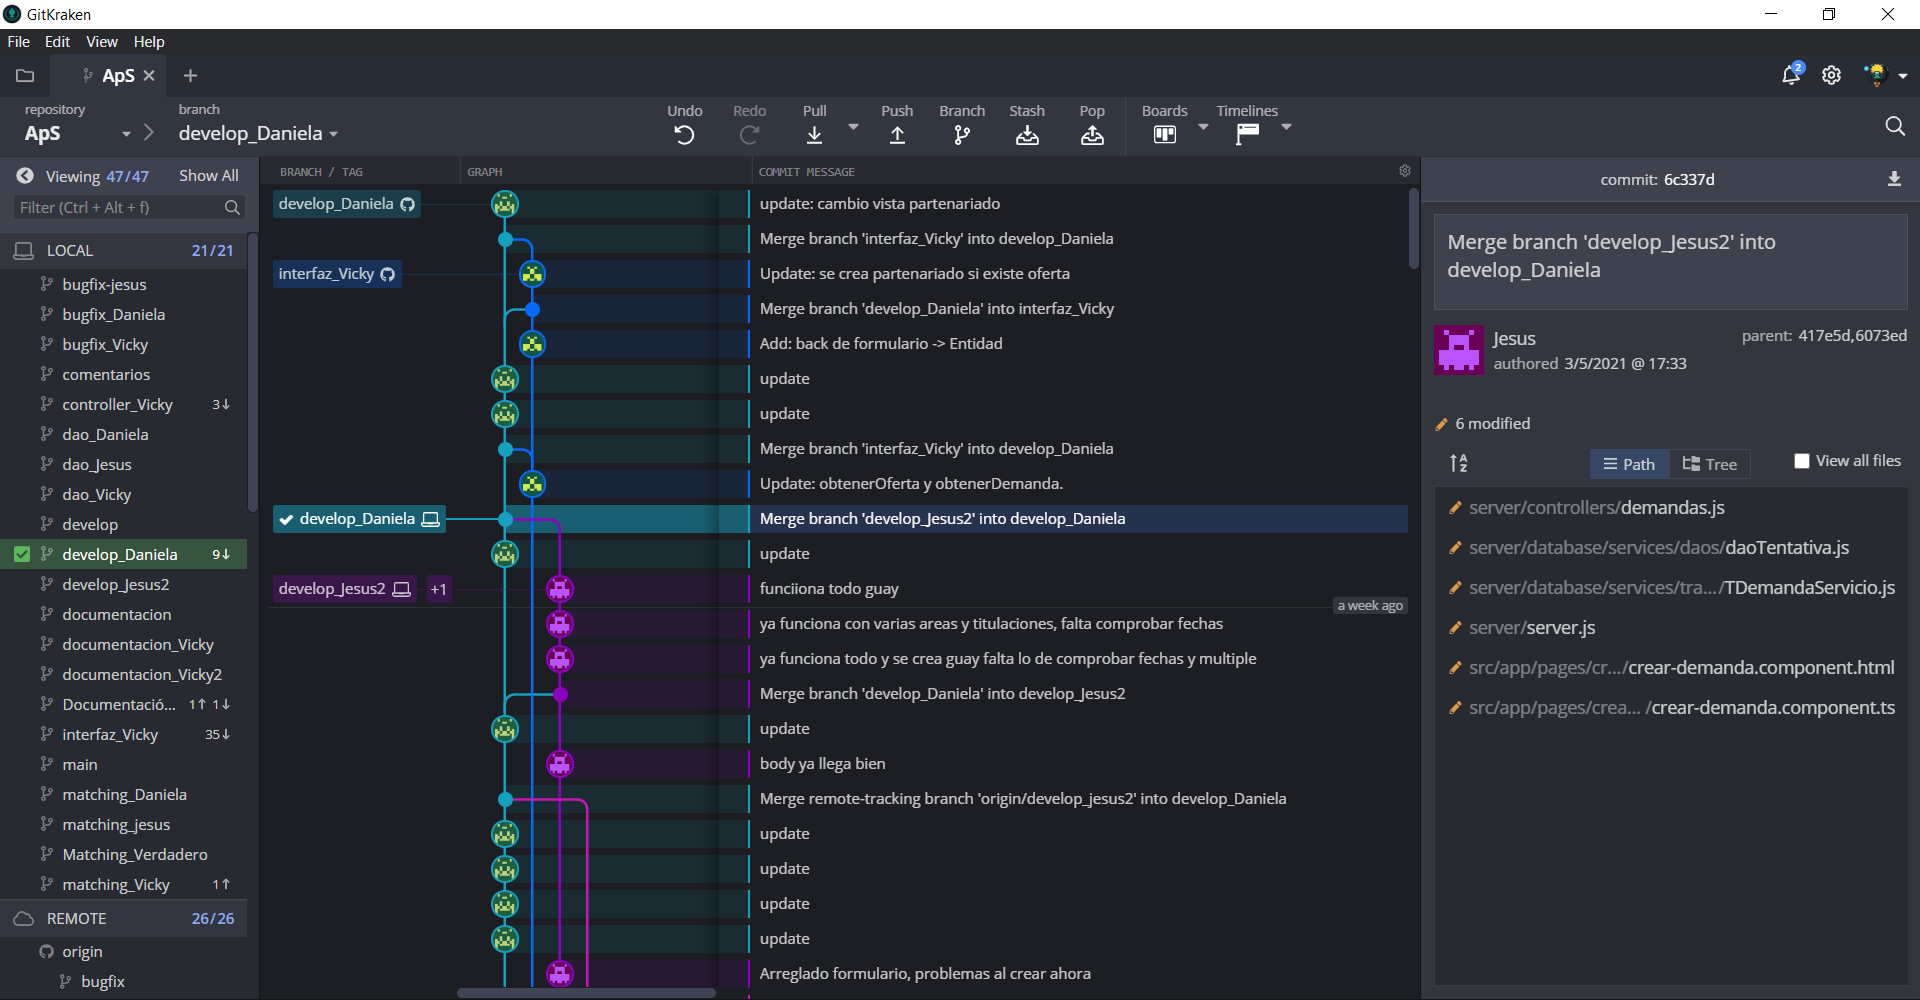
\includegraphics[scale=0.4]{gitkraken}
		\caption{GitKraken: Información de una rama de desarrollo}
		\label{Figura 1}
	\end{figure}
	
	\subsection{Pivotal tracker}
Pivotal tracker es una herramienta de \emph{product planning} y administración de tareas diseñada para equipos de desarrollo que siguen metodologías de diseño ágiles.
	Esta herramienta permite crear historias de usuario y asignarles una puntuación del 1 al 5 indicando su dificultad y/o tiempo invertido en dichas tareas. Además, permite cambiar el estado de las tareas (empezado, finalizado, en revisión,etc) y cualquier cambio en el estado de dichas tareas se informa por correo de manera automática a quien esté involucrado en ella.
	También permite ver las tareas completadas y rechazadas y generar gráficos indicando el esfuerzo realizado, como el que podemos ver en la figura \ref{Figura 2}. Esta tecnología fue sugerida por Victoria y nos ha facilitado mucho tanto la organización como el seguimiento de nuestros avances.
	
	\begin{figure}
	\centering
	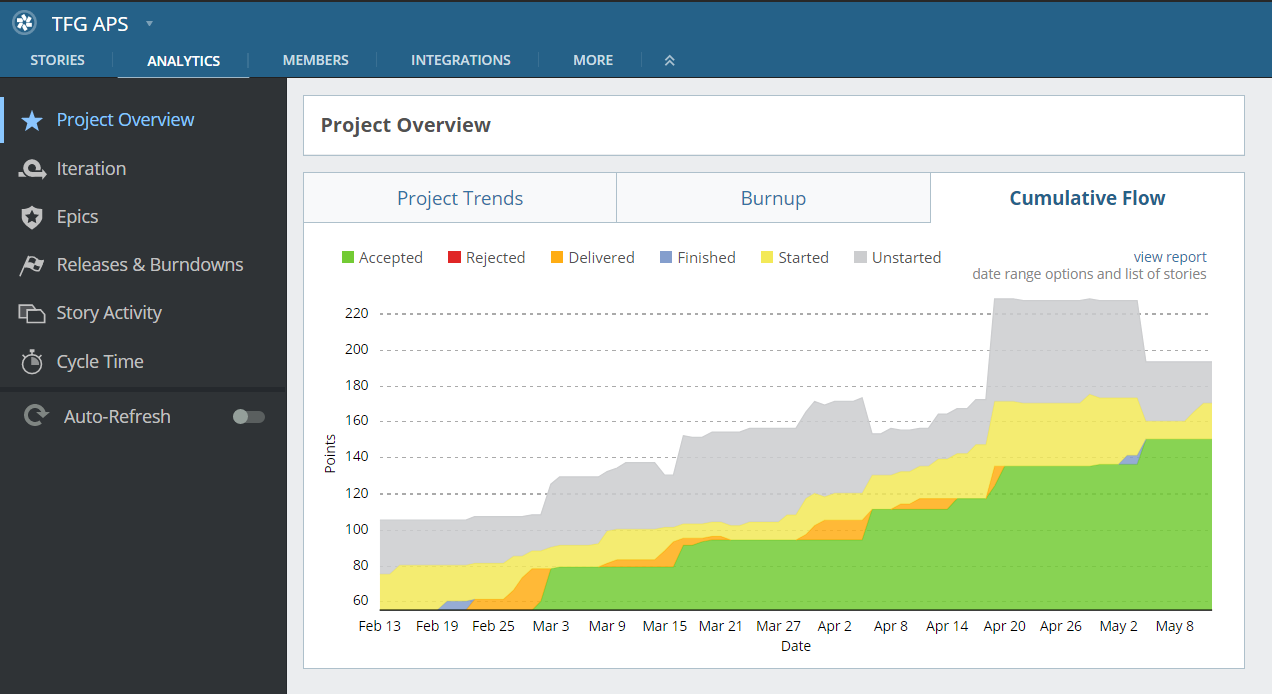
\includegraphics[scale=0.6]{pivotal}
	\caption{Pivotal tracker: Estadísticas de historias}
	\label{Figura 2}
	\end{figure}
	
	\subsection{LaTeX}
LaTeX es un lenguaje de creacion de documentos escritos utilizado comúnmente en el mundo académico, que es una de las principales razones por la que lo hemos escogido para redactar nuestra memoria, a pesar de que ningún integrante del grupo tuviera experiencia previa con ello. A diferencia de otros procesadores de texto, como Microsoft Word o LibreOffice Writer, se escribe el texto plano y se formatea dicho texto con etiquetas. 
	
	\subsection{MySQL}
Aunque nuestro proyecto continúa el trabajo realizado por David Jiménez del Rey, el cual ya contaba con un sistema gestor de bases de datos, dicho sistema era MongoDB. Como los datos que se iban a manejar en la aplicación eran en su mayoría relacionales se tomó la decisión de utilizar MySQL para la base de datos. Dado que todos los componentes del grupo tenían experiencia previa en bases de datos SQL fue un cambio bien recibido.

	\subsection{Modelio}	
Modelio es un entorno de modelado \emph{open-source} el cual permite trabajar con un amplio rango de modelos y diagramas. Dado que ya se contaba con experiencia previa en esta herramienta por parte de todos los miembros del equipo, se ha escogido para realizar los modelos de datos necesarios para la aplicación.
	
	\subsection{MySQL Workbench}
MySQL Workbench: Es una herramienta para diseño, desarrollo y administración de bases de datos relacionales. 
Cuenta con funcionalidades de validación de esquemas y modelos y promueve las mejores prácticas de los estándares de modelado de datos. También promueve los estándares de diseño específicos de MySQL para evitar errores al generar esquemas relacionales o creando bases de datos MySQL. Por estos motivos, junto con su relativa simplicidad es por lo que se ha elegido esta herramienta para hacer los diagramas de entidad-relacion.
	

\section{Modelos (nombre provisional)}
\subsection{Introducción}
Al empezar con el proyecto, junto con nuestros tutores, nos hemos dado cuenta de que la aplicación necesitaba ser definida de una forma más profesional y robusta. David entendió que los profesores y las entidades definían los proyectos de la misma forma, pero esto no es así.\\\\
Las entidades no conocen todos los detalles del problema en cuestión que quieren resolver, porque no suelen dedicarle el suficiente tiempo a la especificación.\\\\
Los profesores por su parte tienen una idea muy vaga del problema que quieren resolver. Normalmente tienen ciertos conocimientos académicos los cuales quieren aplicar para mejorar el mundo, pero la necesidad social en cuestión no suele estar muy clara.\\\\
David creó un elemento llamado Iniciativa que almacenaba algunas de las características generales que comparten las dos propuestas y derivaba en un formulario que se les ofrecía a las entidades y a los profesores. Pero debido a que las entidades y los profesores no plantean los problemas de la misma manera, no es apropiado presentarles el mismo formulario.\\\\
Para definir con precisión el funcionamiento correcto y completo de la aplicación, se ha creado un modelo de dominio y un modelo de datos.\\\\
Estos modelos nos permitirán entender acertadamente el funcionamiento del aplicativo, pero lo que es más importante, permitirán transmitir dicho funcionamiento e idea general a otras personas que trabajarán en este proyecto después de nosotros.\\\\
Gracias al modelo de dominio podemos entender que elementos intervienen y cómo interactúan entre sí, además de las restricciones que se presentan en sus interacciones.\\\\
Con el modelo de datos podemos conocer información detallada de cada elemento que interviene en la resolución del problema.\\\\
Como se ha rediseñado la base de datos, no solo porque ha cambiado su tipo, que ahora es relacional, si no también porque los conceptos no estaban claros en el anterior TFG. Se ha decidido crear un modelo relacional que muestra todas las tablas de la nueva base de datos y sus relaciones. De esta manera podemos representar sus especificaciones técnicas para comprender su estructura y funcionamiento. 

\subsection{Modelo de dominio}
El modelo de dominio es un mapa conceptual del aplicativo que permite a cualquier individuo entender su funcionamiento.\\\\
Si empezamos mirando nuestro modelo desde arriba podemos observar que hay una clase padre llamada usuario y de ella se ramifican otras 5 clases que representan los 5 grupos de usuarios que tiene la aplicación.\\
Los estudiantes se dividen en internos y externos. Los internos representan a aquellos estudiantes que pertenecen a la UNED y los externos pertenecen a otras universidades.\\
El grupo de usuarios promotor se divide en externos e internos por el mismo motivo que los estudiantes. \\
En promotor externo representaríamos al profesor externo, que es aquel profesor que no forma parte de la UNED pero, puede participar en un proyecto o partenariado evaluando y guiando a un estudiante externo. \\
El colaborador por otra parte, es un experto en algún tema en concreto que puede participar en un proyecto o partenariado ofreciendo sus conocimientos o habilidades.\\
El promotor interno puede ser un profesor o un tutor de la UNED. Este profesor es el que más cargos de responsabilidad tiene, él es el que puede crear las ofertas de servicio y es el responsable de los partenariados y los proyectos.\\\\
Todo proyecto tiene que empezar siendo un partenariado y este partenariado se origina en la unión de una oferta creada por un profesor, y una demanda creada por una entidad. La creación de la oferta y la demanda se realiza mediante unos formularios en la web.\\
Una demanda se puede llegar a crear gracias a un estudiante, este previamente ha tenido que crear una iniciativa. Una iniciativa es una propuesta de proyecto de un estudiante, la cual es acogida posteriormente por una entidad. Cuando la entidad acoge dicha iniciativa esta se convierte en una demanda de servicio.\\
Debido a que los proyectos definidos por los profesores y los definidos por las entidades comparten ciertas características, podemos ver en el diagrama que ambos cuelgan de un elemento padre llamado Anuncio de servicio que posee las características comunes de ambos.
Lo mismo ocurre con partenariado y proyecto que cuelgan de Colaboración Uni-Ent.\\
Queremos destacar, que los atributos de Necesidad social y Area de implementación, tan importantes para caza de ofertas y demandas, han sido obtenidos de la página web www.eoslhe.eu/resources/
Los partenariados y los proyectos presentan ciertas restricciones relacionadas con la participación de alumnos y promotores externos.\\\\
En los proyectos solo pueden participar estudiantes externos si el responsable del proyecto acepta estudiantes externos. 
Los profesores externos solo pueden participar en aquellos partenariados y proyectos que los acepten, ademas el proyecto tendrá que admitir estudiantes de la misma universidad que el profesor para que puedan ser evaluados por este.\\\\
\begin{figure}
	\centering
	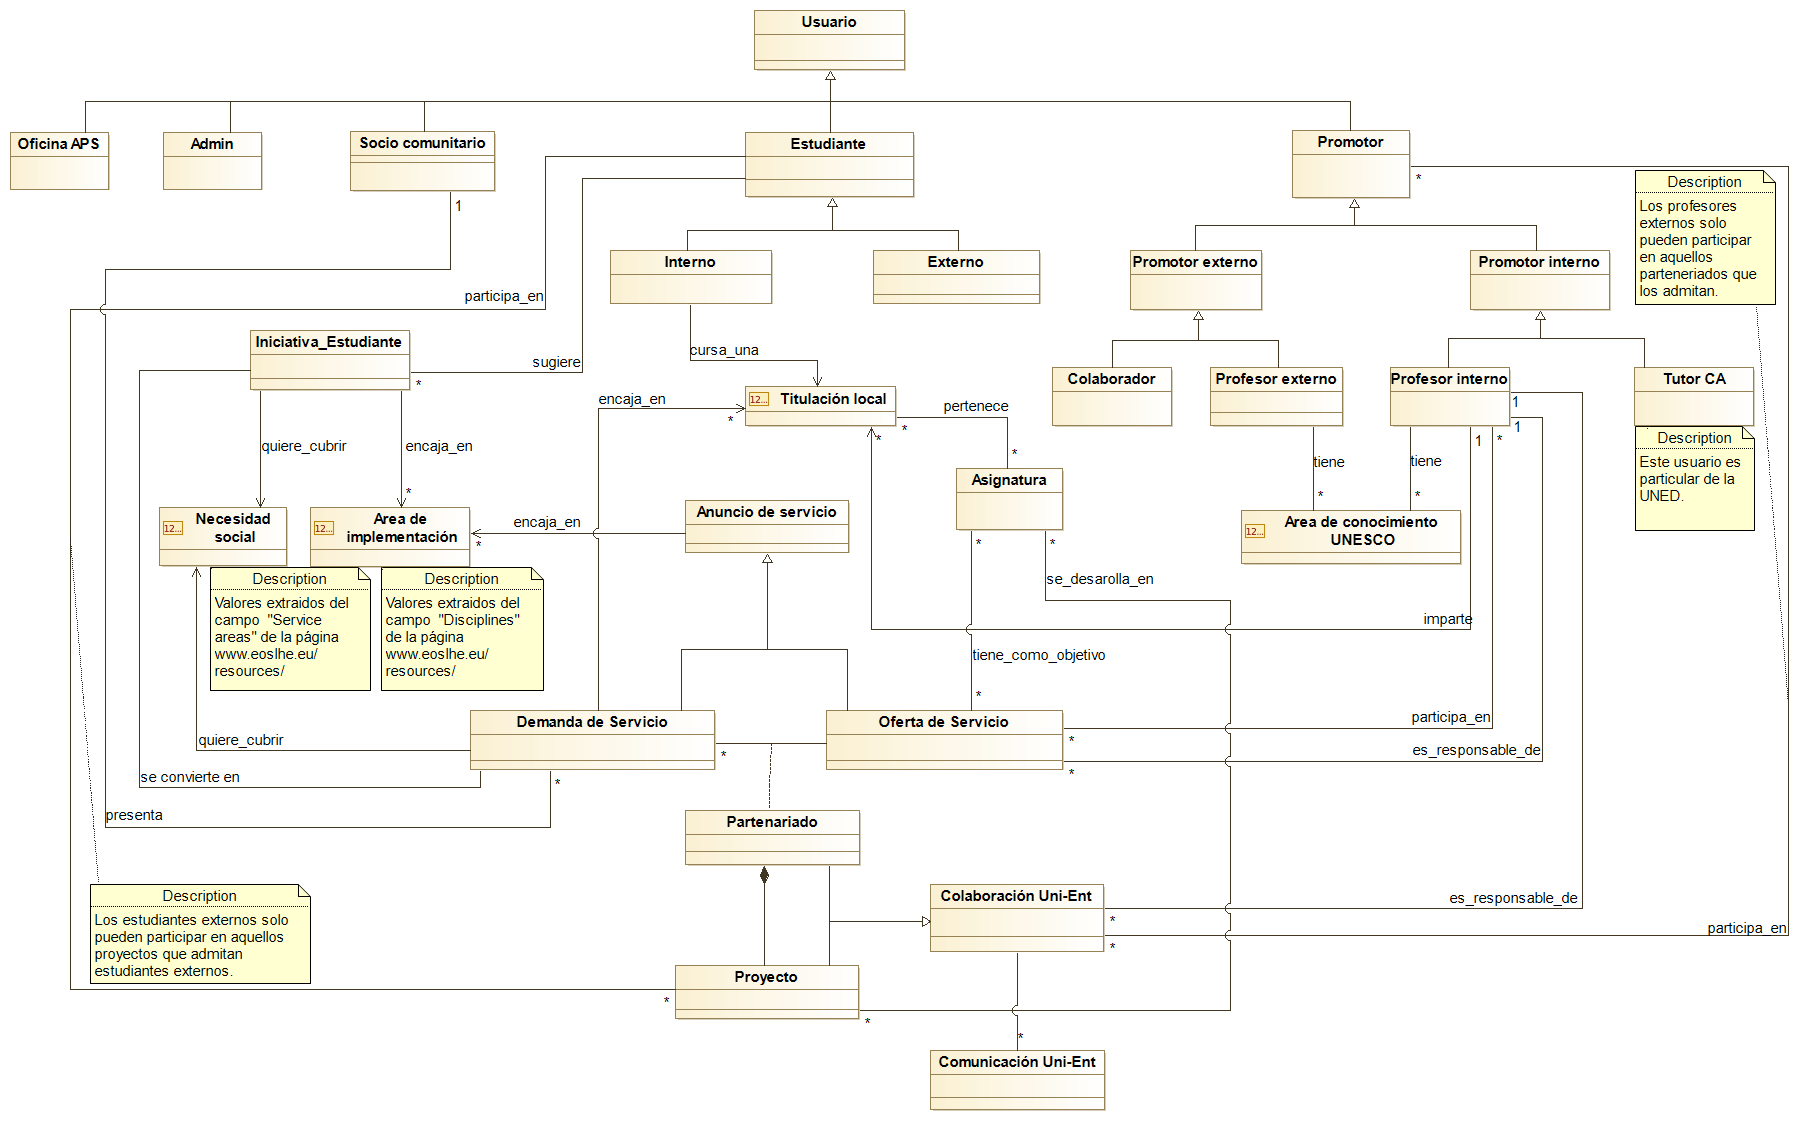
\includegraphics[scale=0.23]{mdominio}
	\caption{Modelo de dominio}
\end{figure}
\begin{figure}
	\centering
	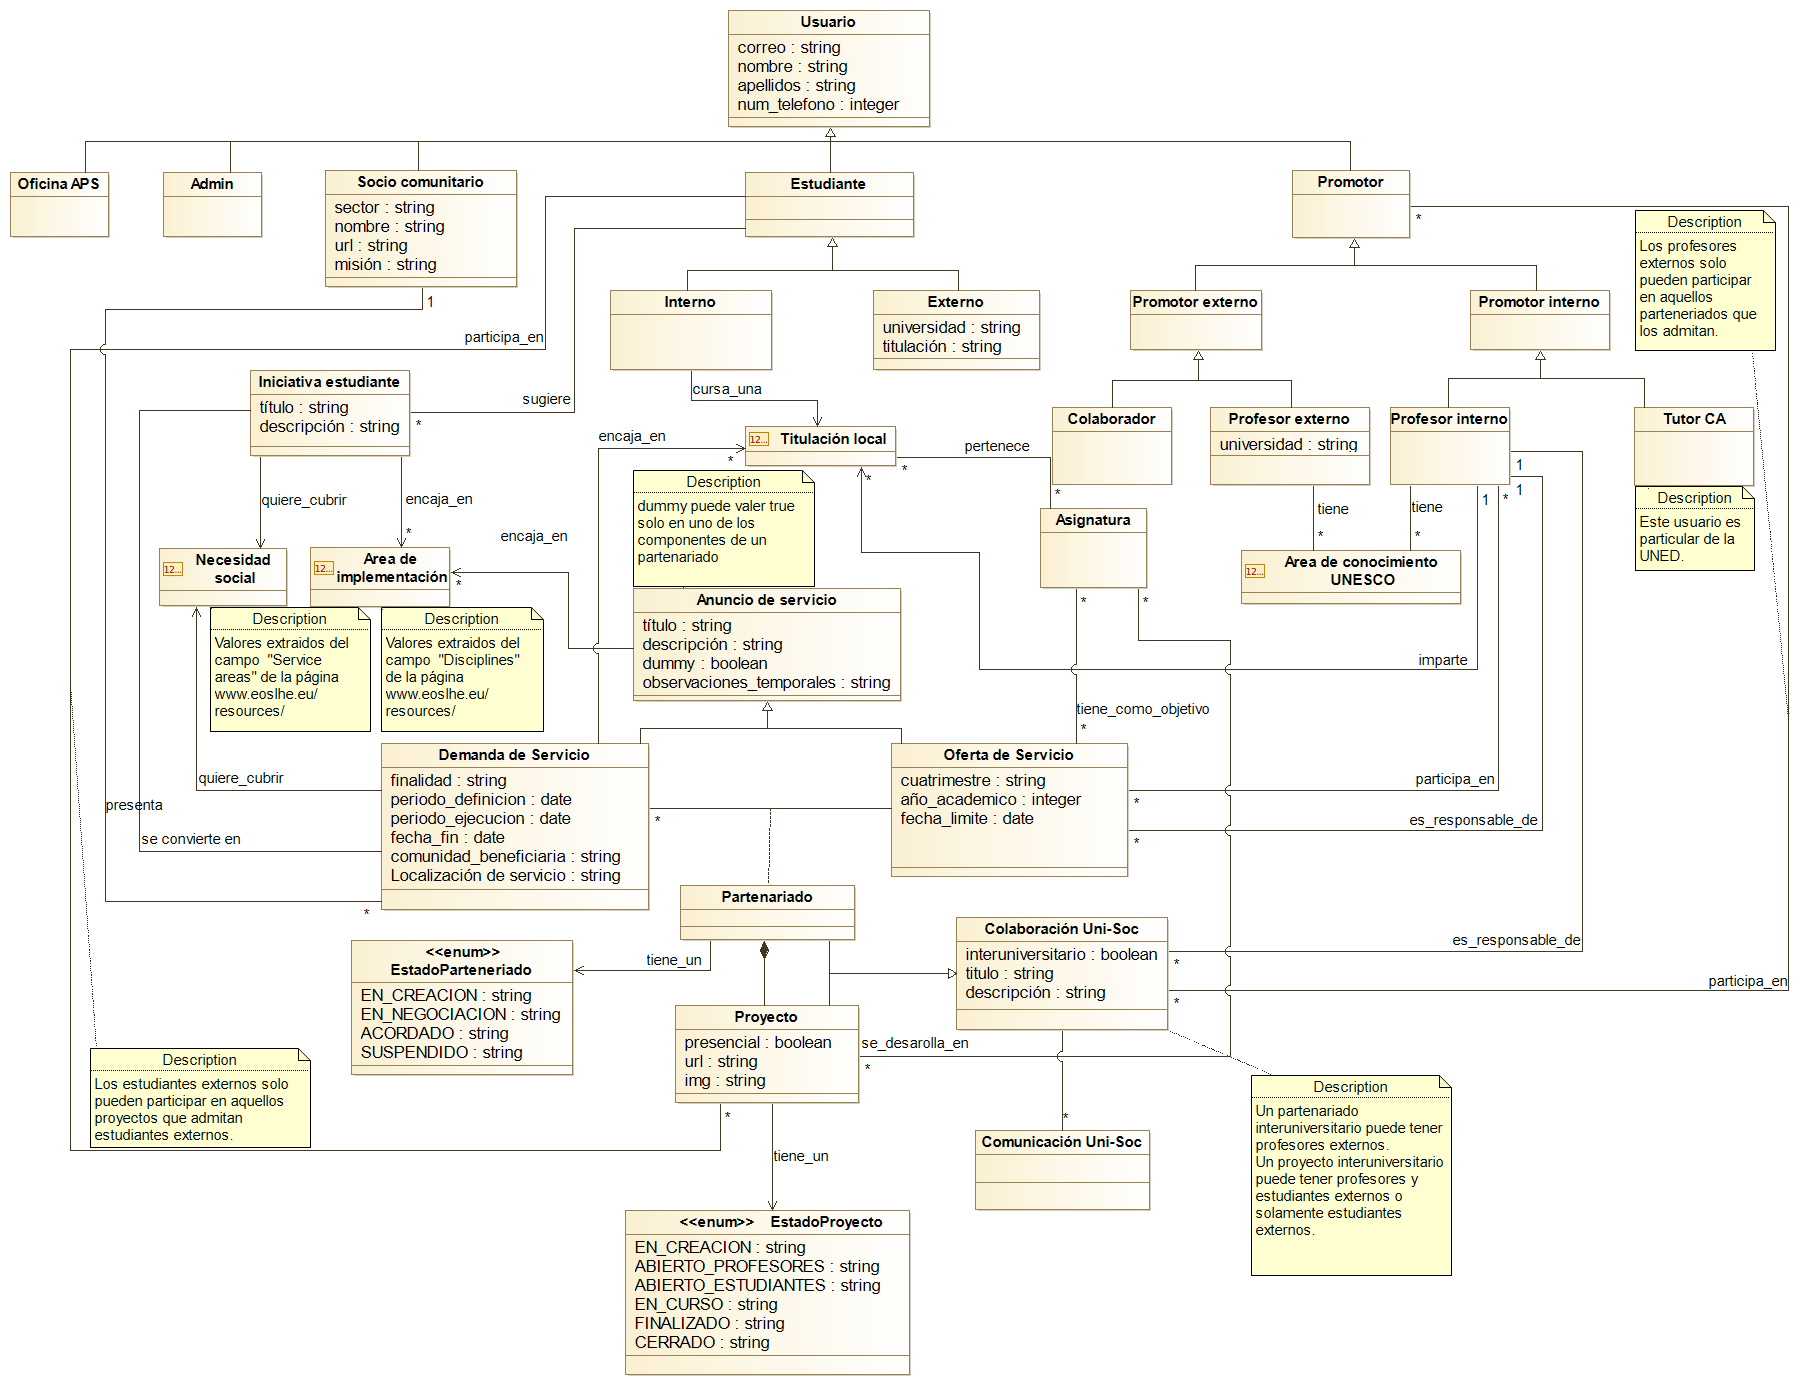
\includegraphics[scale=0.23]{mdatos}
	\caption{Modelo de datos}
\end{figure}
\subsection{Modelo de datos}
El modelo de datos describe con más precisión el dominio de la aplicación.
Además de algunos atributos importantes como el interuniversitario que indica si el partenariado o el proyecto está abierto a externos, podemos observar los estados que pueden tener el partenariado y el proyecto representados por dos enumerados.\\\\

En particular podemos ver que el partenariado puede encontrarse en estados EN\_CREACION, EN\_NEGOCIACION, ACORDADO y SUSPENDIDO.\\ 
El partenariado toma el estado de EN\_CREACIÓN cuando el profesor se pone en contacto con la entidad, si la entidad contesta y acepta aliarse con el profesor el estado del partenariado pasará a EN\_NEGOCIACION. Cuando el profesor y la entidad terminan de establecer los términos y condiciones del partenariado y ambos están de acuerdo el partenariado pasá a estar ACORDADO. Si ocurre cualquier discrepancia durante la fase de EN\_CREACION, EN\_NEGOCIACION o ACORDADO el partenariado puede pasar al estado de SUSPENDIDO.\\\\

En el caso del proyecto tenemos los estados EN\_CREACION, ABIERTO\_PROFESORES, ABIERTO\_ESTUDIANTES, EN\_CURSO, FINALIZADO y CERRADO.
Cuando el profesor decide seguir con el proyecto debe rellenar un formulario, al rellenar dicho formulario el estado del proyecto pasa a estar EN\_CREACION. La entidad recibe dicha solicitud de continuación y debe rellenar otro formulario, una vez rellenado y enviado el proyecto pasa al estado de ABIERTO\_PROFESORES. Una vez que el proyecto ha sido definido se abre a los alumnos y es allí cuando el proyecto pasa al estado de ABIERTO\_ESTUDIANTES. Si el proyecto finaliza correctamente pasará al estado de FINALIZADO. Si sucede cualquier imprevisto durante las 4 fases anteriores el proyecto puede pasar al estado CERRADO.

\subsection{Modelo relacional}

 Debido a la complejidad de la nueva base de datos compuesta por 46 tablas relacionales, se ha decidido crear un diagrama que sirva como mapa en la gestión de la base de datos.\\\\
Este modelo relacional se divide en 4 secciones claramente diferenciadas.\\
La sección de los usuarios que contiene tablas relacionadas con información de los usuarios. La sección del Anuncio de servicio que contiene todas las tablas que representan información de la oferta de servicio, la demanda de servicio y la iniciativa.
La sección de Colaboración contiene la información relacionada con el partenariado y el proyecto.
Y la última es la sección que tiene menos complejidad, la sección de Comunicación que contiene las tablas de \textit{mail}, mensaje, \textit{upload} y \textit{newsletter}, estas creadas por David que se han mantenido intactas.
\begin{figure}
	\centering
	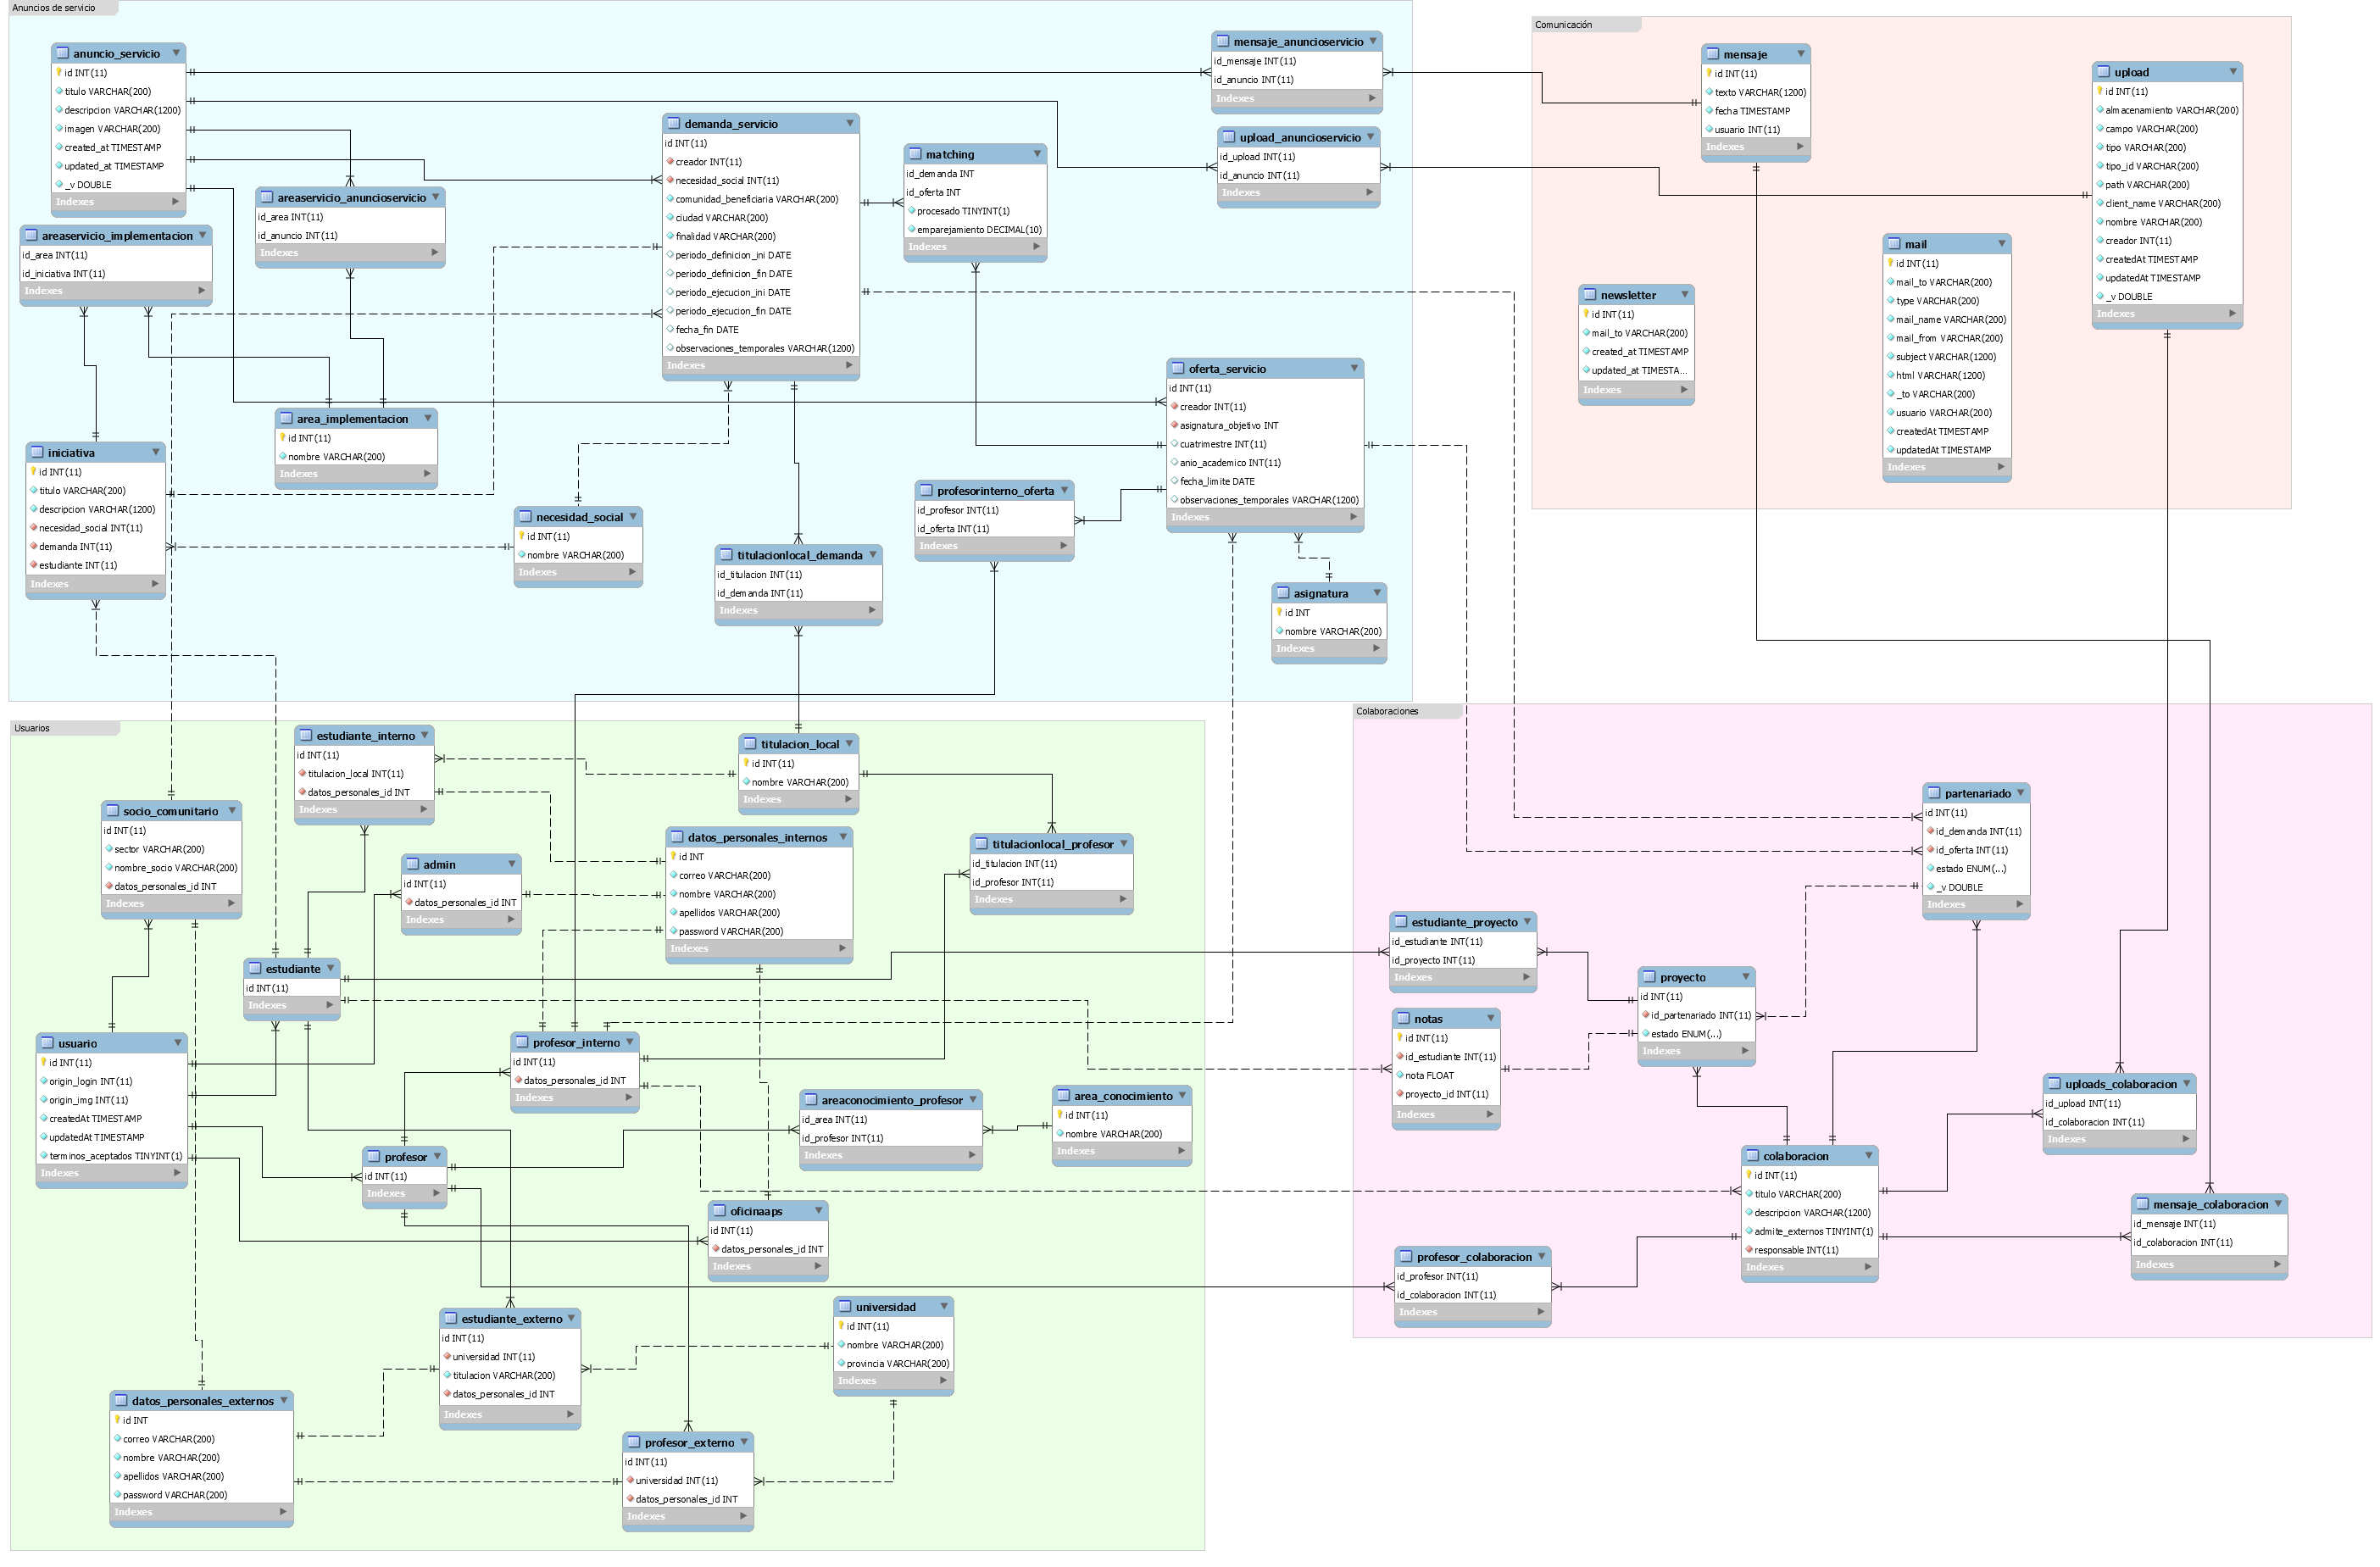
\includegraphics[scale=0.15]{er}
	\caption{Diagrama de entidad relación}
\end{figure}
\subsubsection{Usuarios}
Esta sección es la más compleja debido a la separación que hay que realizar de los usuarios externos e internos.\\
Un usuario interno es aquel profesor, tutor, colaborador, estudiante o representante de la oficina ApS que forma parte de la universidad en la que se despliega la plataforma y por tanto tiene sus datos personales dentro de ella. Debido a que estos tienen parte de los datos que necesitamos para la aplicación en el sistema interno de la universidad hay que tratarlos de manera diferente a los usuarios externos, que son aquellos que no pertenecen a la universidad. Los colaboradores y tutores que aquí mencionamos se pueden ver representados en el modelo de datos y de dominio, pero no se observan aquí porque no nos dio tiempo a integrarlos en la base de datos.\\\\
Debido a esta separación, todos los usuarios comparten una tabla común llamada usuario que contiene datos exclusivos de la cuenta de la plataforma. Después tenemos tablas que contienen datos particulares de cada tipo de usuario, estas son las tablas de entidad, estudiante interno, estudiante externo, \textit{admin}, profesor interno, profesor externo y oficina ApS.\\
Cada uno de estos usuarios poseen una tabla que almacena sus datos personales haciendo diferenciación entre internos y externos. La tabla de datos\_personales\_internos es una tabla creada para la simulación de la aplicación, una vez la aplicación sea desplegada en un entorno real esta tabla será eliminada y los datos personales se obtendrán haciendo consultas a la base de datos de la universidad.\\
Después podemos observar tablas secundarias que representan características de los usuarios como es, la universidad del profesor y estudiante interno, las Áreas de Conocimiento UNESCO de los profesores y las titulaciones que imparten los profesores o cursan los alumnos.
\begin{figure}
	\centering
	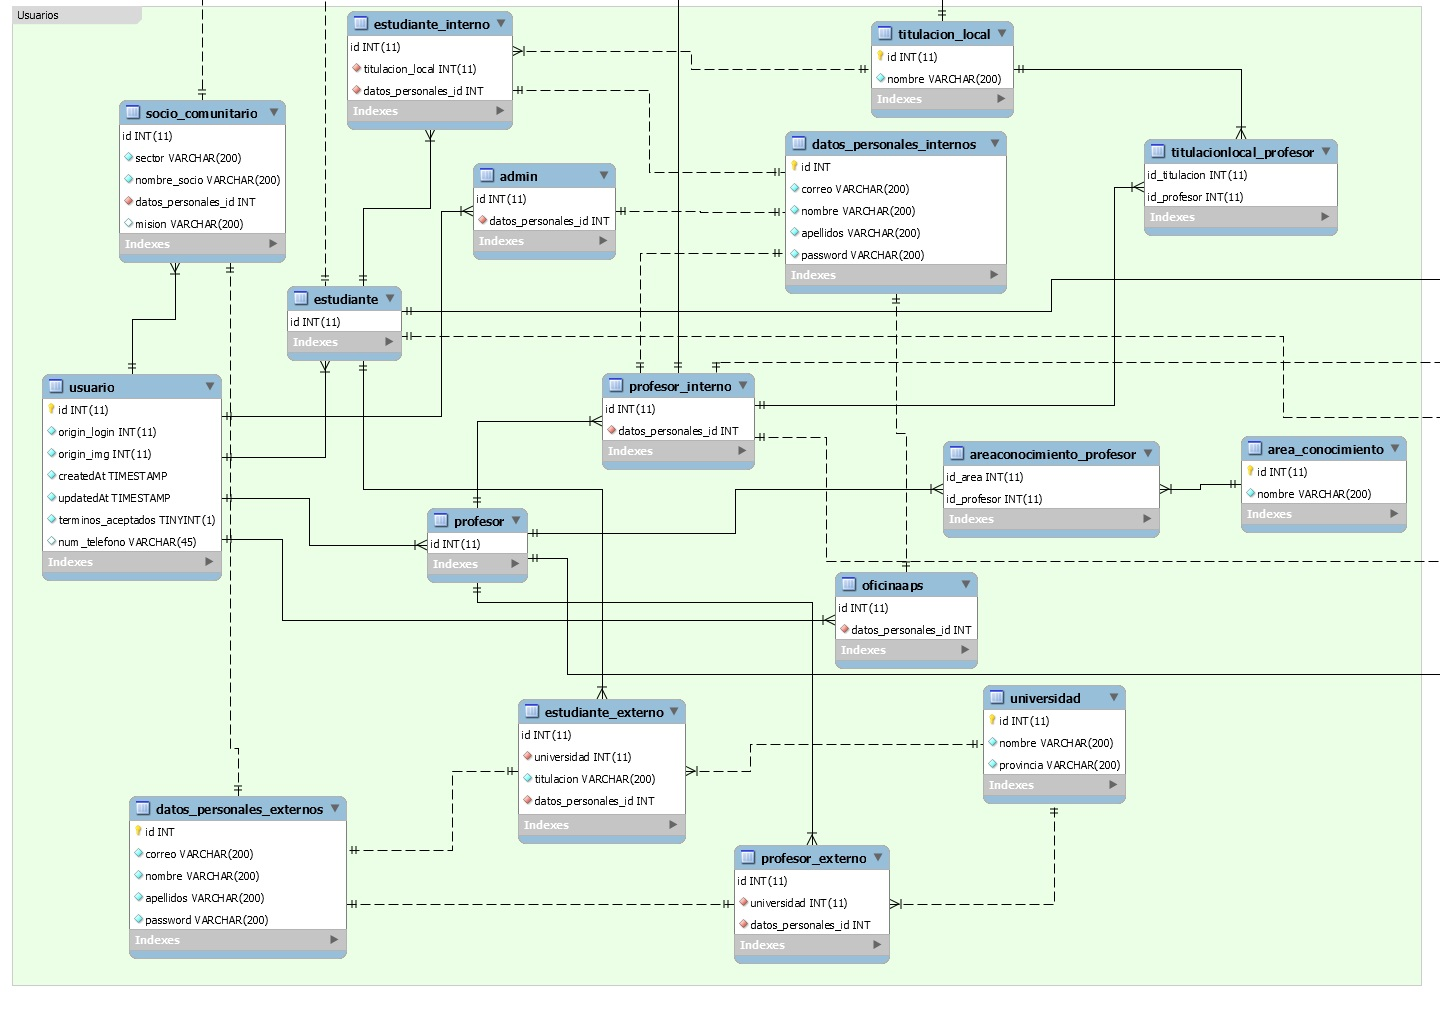
\includegraphics[scale=0.4]{usuarios}
	\caption{Diagrama de entidad relación: Usuarios}
\end{figure}
\subsubsection{Anuncios de servicio}
En este conjunto de tablas podemos encontrar las pertenecientes a la demanda de servicio, la oferta de servicio y la iniciativa.\\
La iniciativa es una propuesta de proyecto realizada por un estudiante. Esta propuesta debe ser validada por un administrador y posteriormente adoptada por una entidad que desee realizar el proyecto.\\\\
La demanda de servicio es creada por una entidad y define una necesidad especifica que quiere cubrir. Esta necesidad social es representada por un enumerado alojado en la tabla de necesidad\_social.
Estos enumerados han sido obtenidos del campo Service areas hallado en la página www.eoslhe.eu/resources/ .
Los enumerados alojados en la tabla area\_servicio también se obtuvieron de esta página, del campo llamado Disciplines.\\\\
La oferta de servicio es creada por un profesor interno y tiene menos detalles que la demanda porque es una propuesta más genérica.\\
Cuando una oferta y una demanda son procesadas por el sistema de \textit{matching} se crea una entrada en la tabla \textit{matching} almacenando los \textit{ids} de ambos elementos y el porcentaje de emparejamiento que tienen.\\
Tanto demanda de servicio como oferta de servicio están conectadas a mensajes y \textit{uploads} porque estos permiten la comunicación con las personas interesadas en las propuestas.
\begin{figure}
	\centering
	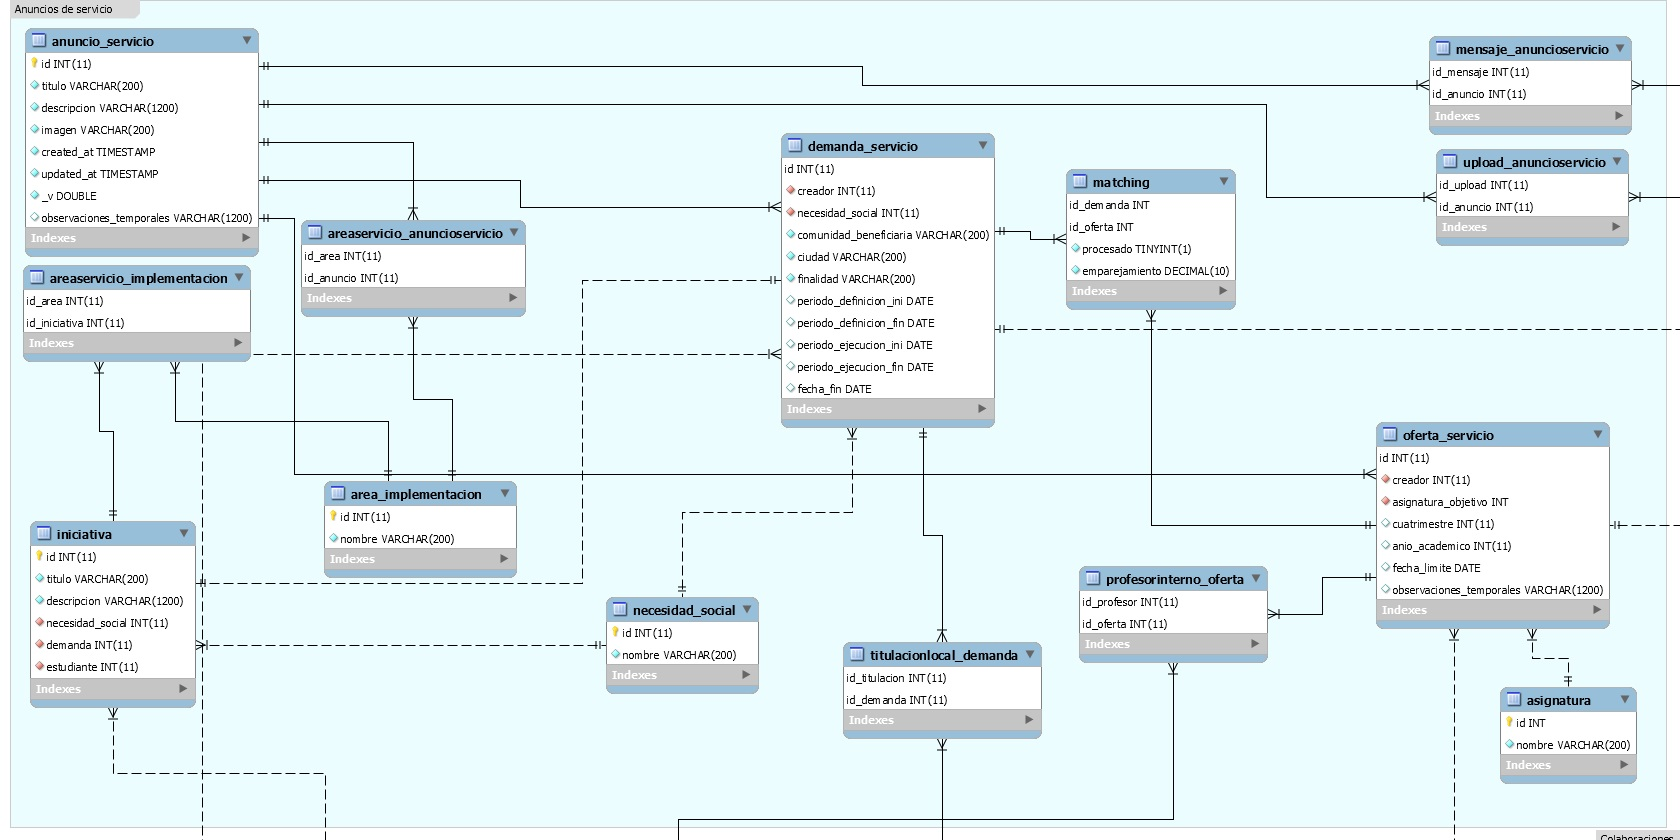
\includegraphics[scale=0.35]{anuncios}
	\caption{Diagrama de entidad relación: Anuncios de servicio}
\end{figure}
\subsubsection{Colaboración}
El partenariado es el segundo paso en la creación de un proyecto, esta tabla contiene las \textit{ids} de la demanda y la oferta que la componen.\\
El proyecto no puede existir sin un partenariado y es por eso por lo que tiene un id del partenariado que lo creó. El proyecto posee estudiantes y es por eso por lo que tiene una conexión con los mismos.\\
Tanto proyecto como partenariado necesitan un sistema de comunicación y es por eso por lo que tienen tablas intermedias que los conectan a mensaje y \textit{uploads}.
\begin{figure}
	\centering
	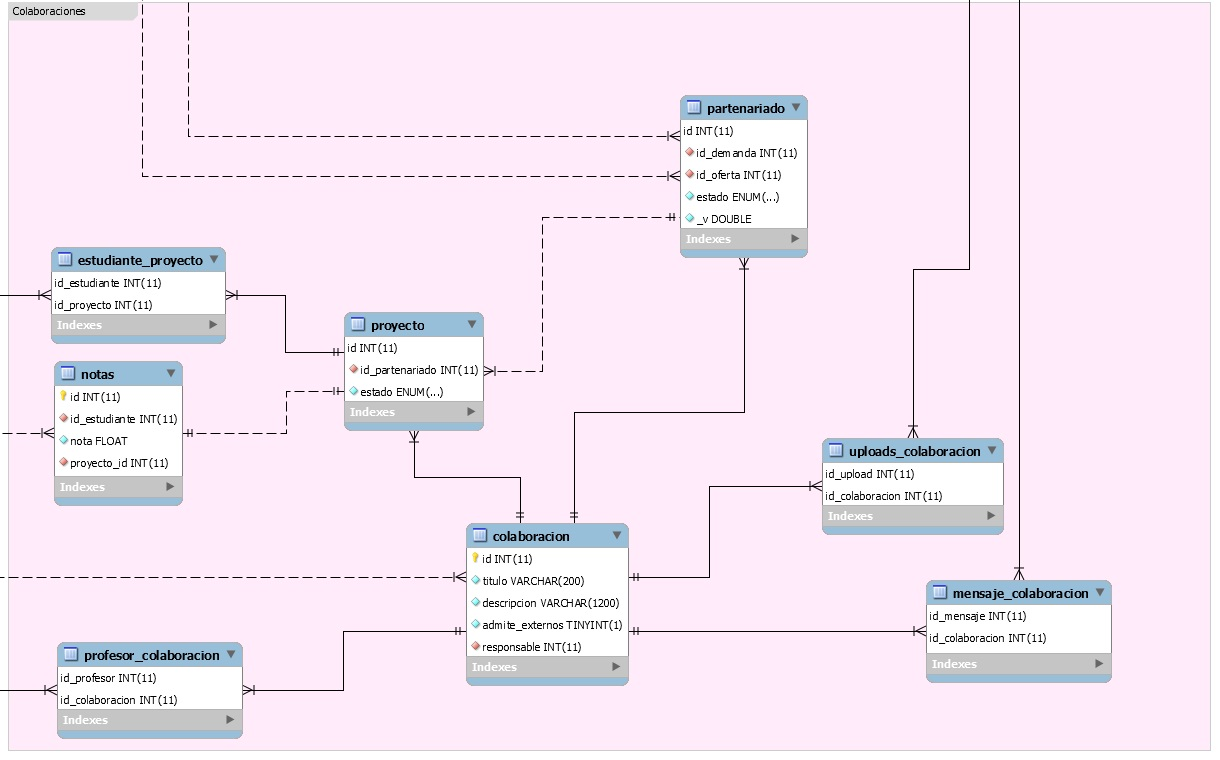
\includegraphics[scale=0.4]{colaboracion}
	\caption{Diagrama de entidad relación: Colaboración}
\end{figure}
\subsubsection{Comunicación}
Esta parte se ha mantenido tal y como la había creado David, solo se ha adaptado al nuevo sistema.\\
La tabla de mensajes conecta con las ofertas de servicio, las demandas de servicio, los partenariados y los proyectos porque todos estos necesitan de los mensajes para poder comunicarse.\\
La tabla \textit{upload} almacena la información de los ficheros e imágenes subidos tanto en ofertas de servicio, como demandas de servicio, como partenariados y proyectos.\\
La tabla \textit{mail} y \textit{newsletter} no han sido conectadas con nada porque no se han tenido en cuenta para el desarrollo de este TFG pero representan los correos electrónicos internos de la aplicación y las noticias periódicas enviadas a los usuarios.
\begin{figure}
	\centering
	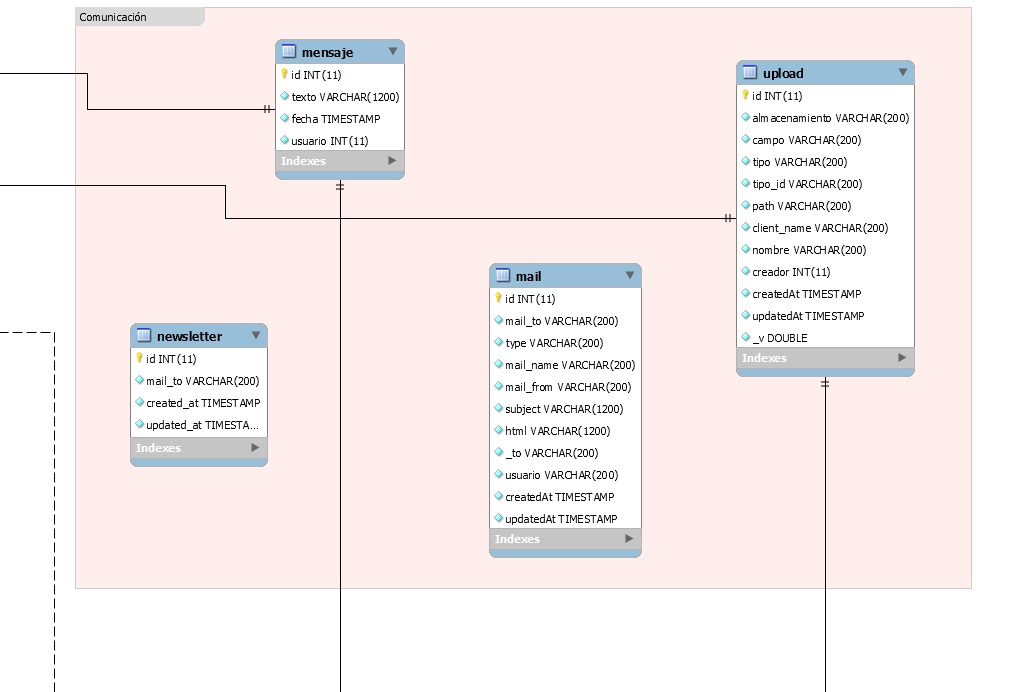
\includegraphics[scale=0.4]{comunicacion}
	\caption{Diagrama de entidad relación: Comunicación}
\end{figure}

\section{Capa de acceso a datos}

Tras cambiar la base de datos de MongoDB por una relacional, también era necesario hacer la lógica de accesos a la base de datos, por lo que se crearon cuatro \emph{Data Access Object} (DAO a partir de ahora) que se encargarían de las operaciones de cada una de las cuatro áreas definidas en el modelo de entidad-relación.

El DAO es un patrón de diseño el trata de proporcionar una interfaz para la comunicación con una base de datos u otro sistema de persistencia de datos. Esta interfaz se encarga de llevar a cabo las operaciones CRUD, es decir creación, lectura, actualización y eliminación de datos y además asegura la independencia entre la lógica de la aplicación y la capa de negocio.

Aunque no eran estrictamente necesarios dado que en javascript no hace falta declarar el tipo de los objetos, se decidió crear objetos \emph{transfer} para así tener más documentados los campos de cada tipo de objeto.
Un \emph{transfer} o \emph{Data Transfer Object} es un objeto cuya única función es guardar la información de cierto objeto y permitir su acceso y manipulación.
De esta forma si hay algún problema, este se detectará cuanto antes y evitará que la aplicación falle repentinamente más avanzada su ejecución.

Los objetos \emph{transfer} contienen simplemente los atributos deseados de cada tipo de objeto además de las funciones \emph{get} y \emph{set} para poder acceder y actualizar la información de dichos atributos.
En conjunto con los DAO, los \emph{transfer} ayudan aún más a la separación de capas de negocio y lógica.

Los cuatro DAO que se crearon a partir del diagrama entidad-relacion son:

\begin{itemize}
	\item \texttt{DAOColaboracion}: Se encarga de manejar toda la información relacionada con los proyectos y los partenariados, desde sus participantes, ya sean profesores o alumnos hasta los mensajes y archivos asociados a estos proyectos o partenariados. Este DAO se llama así porque tiene como piedra angular la clase \texttt{Colaboración}.
	Esta clase fue creada para hacer de padre de las clases \texttt{Partenariado} y \texttt{Proyecto} y así evitar la repetición de métodos y atributos similares. Utiliza los \emph{transfer} \texttt{TColaboracion}, \texttt{TPartenariado} y \texttt{TProyecto}.

	\item \texttt{DAOComunicacion}: Se encarga de manejar toda la información relacionada con todas las formas de comunicación disponibles, desde los mensajes y los \emph{uploads} que se pueden intercambiar durante las distintas fases de un partenariado o proyecto hasta los \emph{emails} o las \emph{newsletter} a las que se pueden suscribir los usuarios. Por lo tanto utiliza los \emph{transfer} \texttt{TUpload}, \texttt{TMensajes}, \texttt{TMail} y \texttt{TNewsletter}

	\item \texttt{DAOTentativa}: Se encarga de manejar toda la información relacionada con ofertas y demandas y sus relaciones con la titulación local ofrecida por la universidad, las áreas de servicio y las necesidades sociales que pudiera tener la demanda. 
	Al igual que antes, se creó una clase padre llamada \texttt{Anuncio} para evitar la repetición de atributos en las clases \texttt{Oferta} y \texttt{Demanda} y en sus derivadas. Este DAO también se encarga de las iniciativas, que son propuestas de proyecto realizadas por un alumno a la espera de que se le dé el visto bueno, y de los mensajes y \emph{uploads} que pudieran tener tanto la oferta como la demanda. Para poder llevar a cabo esta función, este DAO utiliza los \emph{transfer} \texttt{TIniciativa}, \texttt{TOfertaServicio}, \texttt{TAnuncioServicio} y \texttt{TDemandaServicio}.

	\item \texttt{DAOUsuario}: Se encarga de manejar los datos pertenecientes a las distintas clases de usuario, que son: profesor interno, profesor externo, estudiante interno, estudiante externo, \emph{admin}, socio comunitario y oficina APS.
	Además de estas clases también interactúa con los respectivos padres de cada una de ellas y con las titulaciones locales, áreas de conocimiento y universidades que son necesarias para completar los atributos de los profesores.
	Para ello utiliza los \emph{transfer} \texttt{TAdmin}, \texttt{TEntidad} (que deberá cambiarse en un futuro por \texttt{TSocioComunitario}), \texttt{TUsuario}, \texttt{TProfesor}, \texttt{TOficinaAPS}, \texttt{TEstudiante}, \texttt{TProfesorExterno}, \texttt{TProfesorInterno}, \texttt{TEstudianteInterno} y \texttt{TEstudianteExterno}.

	
	\end{itemize}
	Se ha intentado que los DAO tengan todas las funcionalidades necesarias para que la aplicación pudiera seguir funcionando tras sufrir cambios sin necesidad de actualizar los DAO con frecuencia, pero resulta imposible saber qué nuevas funcionalidades puede adquirir la aplicación o que cambios podría sufrir el modelo de datos así que, aunque cuenta con bastantes funcionalidades, será necesario actualizarlo sobre la marcha si en un futuro la aplicación sufre cambios.

\section{Creación de formularios}
Una vez adaptada la base de datos de no relacional a relacional y creados los correspondientes operaciones CRUD de las tablas, hemos pasado a la creación o a la adaptación de los formularios con los nuevos datos que les corresponde a cada uno de ellos. Para ello, tuvimos que aprender y experimentar con Angular JS, framework de javascript, que requiere un vasto conocimiento para el desarrollo de los formularios y de los archivos para el correcto funcionamiento de estos. 
\subsection{Formulario de registro de usuarios}
El primer formulario que tuvimos que tratar fue el registro de usuarios, siendo este el punto de inicio para los posteriores formularios a crear.\\\\
En el TFG de David ya venía un registro implementado con sus correspondientes campos, pero al probar la aplicación habíamos encontrado algunos errores que tuvimos que corregir. Uno de los errores que encontramos era que permitía introducir una contraseña no robusta de cualquier longitud y sin ninguna restricción. De manera que la hemos hecho más robusta con una longitud mínima de 8 caracteres, mínimo una mayúscula, mínimo una minúscula y mínimo un carácter especial. También el campo email no verificaba si era uno  correcto, de modo que tuvimos que crear las validaciones correspondientes por si no contenía el “@” o el “.” .\\\\
En el formulario de David existían dos campos para la contraseña: contraseña y repetir contraseña, donde ambos campos deben contener el mismo contenido para que se pueda permitir la validación del formulario y la creación del usuario, en cambio al pedir la contraseña repetida si se introducía una contraseña distinta al campo de “contraseña “ lo aceptaba y se procedía al proceso de registro. Por eso tuvimos que añadir la validación y los mensajes de error correspondientes para que no se permita el registro si los dos campos no son iguales.\\\\
Una vez arreglados los errores, añadido las mejoras y las nuevas validaciones del registro tuvimos que añadir los campos nuevos correspondientes a cada tipo de usuario de la base de datos. \\\\
En el formulario de registro se permite la elección de tres tipos de usuarios externos: profesor externo, estudiante externo, entidad.\\\\
Para la entidad aparte de los campos ya existentes en el formulario se añadió un nuevo campo “nombre entidad” que representa el nombre de la entidad principal que creará el formulario.\\\\
En el caso del estudiante externo no se han añadido nuevos campos en el formulario, pero si el cambio de funcionalidad del campo universidad. Antes en el campo universidad se permitía introducir un texto, pero como eso podía llegar a causar incoherencias en la base de datos puesto que cualquier usuario podría introducir una universidad que no existiese o con algún carácter incorrecto por lo cual se decidió cambiar. De modo que el campo universidad se convirtió en una lista desplegable que permite una única selección por el estudiante de entre ochenta y tres universidades a elegir.  No se permite la validación del registro si no se selecciona alguna universidad de la lista. \\\\
Para el profesor externo se añadió un campo nuevo y se cambiaron las funcionalidades de algunos otros campos. El campo “universidad” tenía el mismo problema que en el caso anterior por lo que se produjo el mismo cambio. Además, tuvimos que introducir un nuevo campo "Área/s de conocimiento" que representa las áreas de conocimiento que tiene el profesor externo a registrar. Este campo es un desplegable que permite la selección múltiple de entre las ciento noventa áreas disponibles que guardamos en la base de datos en la tabla "area conocimiento". Se puede seleccionar entre una o varias áreas de conocimiento y en el caso de que se haya cometido un error al seleccionar un área se permite desmarcar la elección, pero no se permite la validación del registro en el caso de que no se haya seleccionado ningún área de conocimiento de la lista.\\\\

\begin{figure}
	\centering
	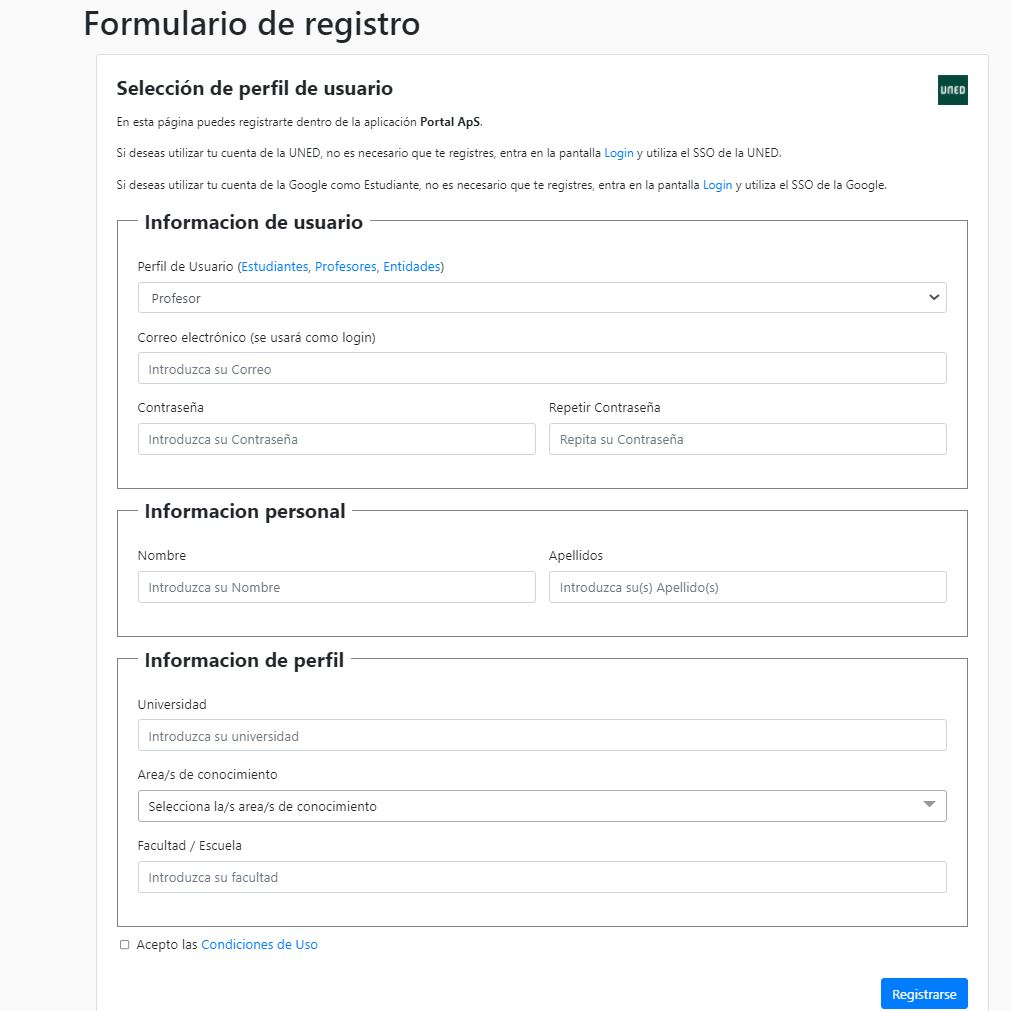
\includegraphics[scale=0.7]{registro}
	\caption{Formulario de registro}
\end{figure}

\subsection{Formulario para editar los datos de un usuario}
En el TFG de David ya existía un formulario para la edición de los datos de un usuario con sus correspondientes campos, pero al cambiar el tipo de base de datos y al introducir nuevos datos en algunos de los tipos de usuarios tuvimos que adaptarlo. \\\\
También añadimos validaciones para los campos como email, contraseña y repetir contraseña. Para el campo email se permitía emails incorrectos sin el “@” o sin el “.” , la contraseña se permitía no robusta y al introducir la contraseña repetida permitía que no fuera igual a lo introducido en el campo contraseña. Una vez añadidas las validaciones se introdujeron los campos necesarios para el formulario en función del tipo de usuario.
Para la entidad a parte de los campos ya existentes en el formulario se añadió el campo “nombre entidad” que representa el nombre de la entidad principal que creará el formulario. Dicho campo viene con el valor ya rellenado, teniendo la posibilidad de cambiar su valor.\\\\
Para el estudiante externo no se han añadido nuevos campos en el formulario, pero si el cambio de funcionalidad del campo universidad, que se convirtió en un desplegable que permite una única selección por el estudiante de una lista de ochenta y tres universidades a elegir.  No se permite la validación de registro si no se selecciona alguna universidad de la lista. El campo  viene con el valor ya relleno, teniendo la posibilidad de cambiar su valor.\\\\
En el caso del profesor externo se añadió un campo nuevo y cambiaron la funcionalidad de algunos otros campos más. El campo universidad cambió de ser un texto introducido por el usuario a ser una lista con las universidades para así no llegar a causar incoherencias en la base de datos. El campo ya viene relleno y se puede cambiar su valor por cualquiera de la lista disponible. Además tuvimos que introducir un nuevo campo “Área/s de conocimiento” que representa las áreas de conocimiento de un profesor. Se puede seleccionar al menos una área de servicio y el valor viene ya relleno con los valores del usuario ya creado.


\subsection{Formulario creación demanda de servicio}
Para poder crear una demanda de servicio en la base de datos que nos permita ejecutar el algoritmo de matching tuvimos que crear el formulario desde cero con sus correspondientes archivos puesto que en el anterior TFG no existía.\\\\
Para ello se tuvo que crear su correspondiente modelo con los campos necesarios para la creación de la demanda:id, titulo, descripcion, imagen, ciudad, objetivo, área de servicio, inicio del periodo de definición, final del periodo de definición, inicio del periodo de ejecución, final del periodo de ejecución, fecha fin, observaciones temporales, necesidad social, titulación local, creador, comunidad beneficiaria, createdAt y updatedAt.\\\\
El creador es la entidad que está conectada en la aplicación y la cual accede a la creación de la demanda de servicio.
Para el formulario de la creación de la demanda de servicio se han creado las validaciones correspondientes para los campos a completar de manera que no se pueda permitir la creación de la demanda si alguno de ellos no es correcto y los mensajes correspondientes a los errores.\\\\
En función del campo se permiten distintos valores acorde a los campos que les corresponden de la base de datos: \\
\begin{itemize} 
	\item Los campos título, descripción, imagen,ciudad,objetivo, necesidad social, comunidad beneficiaria, observaciones temporales permiten introducir texto. 
	\item  Los campos periodoDefinicionIni, periodoDefinicionFin, periodoEjecucionIni, periodoEjecucionFin, fechaFin permiten un valor de tipo fecha.
	\item El campo Área/s de servicio es un desplegable que permite selección múltiple entre un total de setenta y ocho áreas de servicios disponibles en la base de datos en la tabla "area servicio" En el caso de que se haya seleccionado algún área de servicio por error se puede descartar la selección. Hay que seleccionar por lo menos una opción para que se pueda validar el campo correctamente.
\end{itemize}
Una vez completados o seleccionados los campos a completar se comprueba el formulario, y en el caso de que estén todos los campos correctos se valida el formulario y se crea la oferta de servicio insertándose en la base de datos. En caso contrario, se avisa al usuario que los campos no están completados adecuadamente para que este proceda a su corrección.\\\\

\begin{figure}
	\centering
	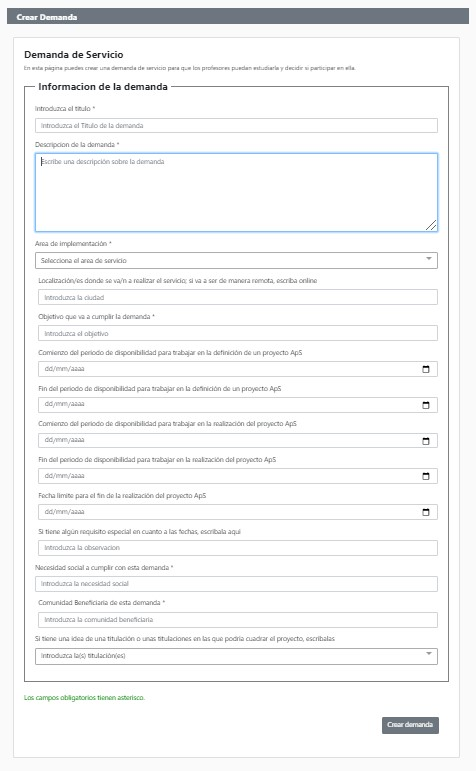
\includegraphics[scale=0.9]{demanda}
	\caption{Formulario de creación de demanda}
\end{figure}

\subsection{Formulario creación oferta de servicio}
Para poder crear una oferta de servicio que sirva para el proceso de matching tuvimos que crear el formulario de creación de una oferta de servicio.En el anterior TFG no existía el formulario, así que tuvimos que crearlo desde cero con sus correspondientes archivos para el correcto funcionamiento en angular js.\\\\
Para ello se tuvo que crear su correspondiente modelo con los campos necesarios para la creación de la oferta: id, titulo, descripcion, imagen, created at, updated at, cuatrimestre, año académico, fecha límite, observaciones, creador, área servicio, asignatura objetivo y profesores. El creador es el profesor interno que está conectado en la aplicación y el cual accede a la creación de la oferta de servicio.\\\\
Para el formulario de la creación de la oferta de servicio se han creado las validaciones correspondientes para los campos a completar de manera que no se pueda permitir la creación de la oferta si alguno de ellos no está correcto y los mensajes correspondientes a los errores. \\\\
En función del campo se permiten distintos valores acorde a los campos que les corresponden de la base de datos: \\
\begin{itemize} 
	\item En los campos título, descripción, asignatura, observaciones temporales se permite introducir texto.
	\item En los campos año académico se permite un valor de tipo numérico que represente un año válido.
	\item El campo fecha límite permite un valor de tipo fecha. 
	\item  El campo cuatrimestre es un desplegable que permite una sola elección entre: Primer cuatrimestre, segundo cuatrimestre y anual. Hay que seleccionar una opción para que se pueda validar el campo correctamente.
	\item El campo Área/s de servicio es un desplegable que permite selección múltiple entre un total de setenta y ocho áreas de servicios disponibles en la base de datos en la tabla “area servicio” En el caso de que se haya seleccionado algún área de servicio por error se puede descartar la selección. Hay que seleccionar por lo menos una opción para que se pueda validar el campo correctamente.
\end{itemize}
Una vez rellenos todos los campos del formulario se procede a su validación, en el caso de estar correcto se almacena la oferta de servicio en la base de datos, en caso contrario se notificará al usuario para que complete de manera correcta los campos erróneos.

\begin{figure}
	\centering
	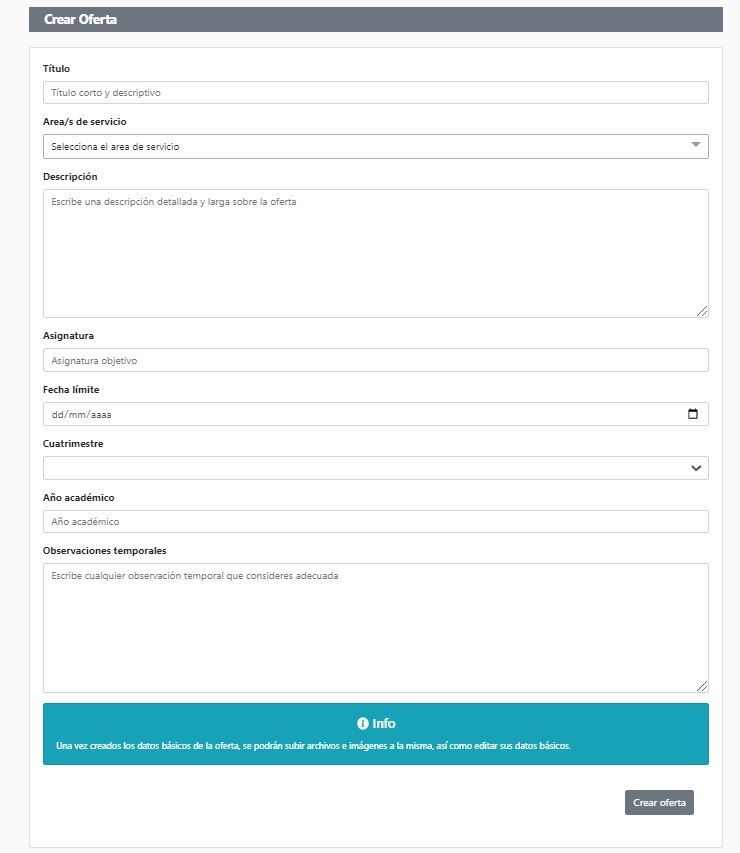
\includegraphics[scale=0.9]{oferta}
	\caption{Formulario de creación de ofertas}
\end{figure}
\subsection{Formulario creación de partenariado profesor}
Una vez creados los formularios de oferta de servicio y demanda de servicio hemos procedido al desarrollo del formulario para la creación del partenariado de un profesor.
El formulario para la creación del partenariado del profesor no existía en el anterior TFG, así que se procedió a su creación desde cero. Para ello, tuvimos que crear los archivos y el modelo necesarios para el formulario. El formulario aparece con unos campos ya rellenos, algunos de los cuales son editables. Se necesitan los datos de la oferta y la demanda en cuestión para poder realizar la creación del formulario.\\\\
En la creación del formulario de partenariado del profesor los datos de la demanda de servicio de la entidad beneficiaria vienen ya completados y sin posibilidad de editarlos En cambio, los datos de la oferta hechos por el profesor responsable que procede a la creación del formulario si tiene la posibilidad de cambiar los datos. Estos datos vienen rellenados con los datos de la demanda de servicio.\\\\
El formulario está dividido en tres partes para la distinción entre los datos generales del partenariado que serán la combinación de los datos en común o los datos más relevantes del formulario, los datos de la oferta y los datos de la demanda. También hemos creado validaciones para todos los campos del formulario, para que no se permitan campos vacíos.\\\\
En el formulario el título y la descripción son una  combinación de los títulos y descripciones de la oferta y la demanda, estos campos son editables. Los datos de la demanda de servicio vienen rellenadas, pero no son editables:  las áreas de servicio,la entidad de la demanda, la localización de desarrollo del partenariado, la finalidad, la comunidad beneficiaria, las fechas, asignatura objetivo, titulaciones locales, cuatrimestre y año académico. Aparece como profesor responsable, el de la oferta, siendo un campo editable que se da a elegir entre una lista de todos los profesores internos de la base de datos.\\\\
El campo equipo de profesores es una lista que da la posibilidad de selección múltiple y viene ya rellenada con los valores de la oferta de servicio ya creada. El profesor que procede a la creación del formulario elige si se aceptan personas externas. El área de servicio de la oferta no es un campo editable. Para que se pueda validar el formulario no deben existir campos vacíos o mal completados, y se mostrarán los mensajes para que informe al usuario de los campos a cambiar o completar. Una vez completado correctamente, al aceptarlo se pasa del estado EN\_NEGOCIACION a EN\_CREACION. Si se rechaza pasa al estado SUSPENDIDO.
\\\\

\begin{figure}
	\centering
	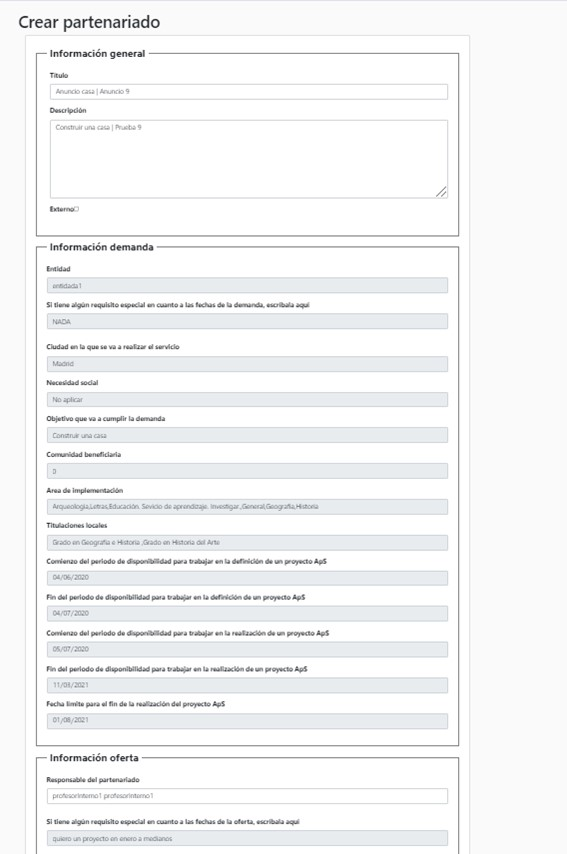
\includegraphics[scale=0.9]{partenariado1}
	\caption{Formulario de creación de partenariado: parte 1}
\end{figure}


\begin{figure}
	\centering
	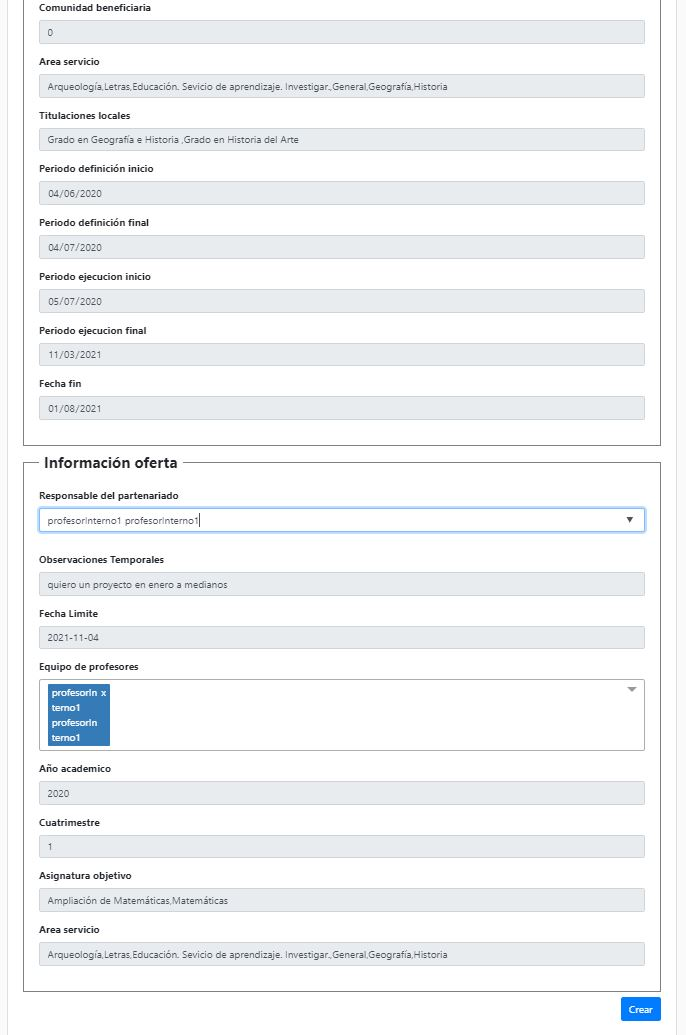
\includegraphics[scale=0.9]{partenariado2}
	\caption{Formulario de creación de partenariado: parte 2}
\end{figure}

\section{Matching entre oferta de servicio y demanda de servicio}

\subsection{Definición del matching }

Para nuestro TFG hemos implementado un algoritmo de matching para las ofertas y las demandas, de manera que cogiendo una oferta y una demanda de la base de datos verificamos si se puede realizar una negociación entre ellas a partir de la información que contiene cada una. Partiendo de unas especificaciones del algoritmo que se estableció entre nosotros y los tutores del TFG, las hemos aplicado para poder obtener la información relacionada representada por un porcentaje, con el cual  se decidirá el resultado final.  Cuantos más datos haya relacionados entre una oferta y una demanda, más porcentaje sacará nuestro algoritmo. El objetivo del algoritmo de matching es ayudar a los profesores a encontrar más fácilmente demandas relacionadas a sus propuestas y a las entidades a obtener ofertas acorde a sus solicitudes. \\\\

Definimos el matching según nuestro algoritmo, como el proceso que consiste en identificar los datos que se ajustan a unos criterios de coincidencia los cuales se van a enumerar a continuación en los siguientes párrafos. De modo que si se encuentran suficientes puntos de similitud entre los datos recopilados, estos son considerados para sacar un porcentaje de coincidencia, donde si este es menor que el valor mínimo establecido no se considerará matching. El valor mínimo que hemos establecido para nuestro algoritmo para considerar la existencia de un matching es 50\%.
\\\\

\subsection{Criterios de matching y anti matching}
\subsubsection{Criterios de matching }

Hemos definido unos criterios en base a los datos proporcionados por los usuarios en las ofertas y demandas de servicio según los cuales se resolverá el matching:

\begin{itemize} 	
	\item Hacer coincidir las descripciones tanto de la oferta como de la demanda de servicio mediante Procesamiento del Lenguaje Natural (NLP).
	Para ello hemos tenido que buscar las palabras comunes del idioma español y almacenarlas en un fichero, para así poder  procesarlas para obtener el resultado deseado. El procedimiento consiste en dadas las dos descripciones, las guardamos en dos estructuras simples de datos, quitamos las palabras comunes (aquellas que sean iguales a las del fichero) y nos quedamos con las que puedan coincidir en las dos descripciones, cada una de estas se guarda en una estructura simple de datos. Al tenerlas, empezamos a procesar las palabras resultantes de las dos descripciones, distinguiendo las mayúsculas, minúsculas, tildes y caracteres especiales, donde obtenemos el número de palabras que coinciden de las descripciones. Para poder obtener el porcentaje de coincidencias, dividimos el número de palabras coincidentes con la descripción que tiene el menor número de palabras. Dicho porcentaje se tendrá en cuenta para poder calcular el matching final.
	
	\item Encontrar la similitud entre las áreas de servicio tanto de la oferta como de la demanda. Se dispone de setenta y ocho áreas de servicio en la base de datos para poder realizar esta comprobación. Para ello se comparan todas las áreas de servicio de ambas, y se devuelve el número de coincidencias. Cuanto mayor dicho número, mayor probabilidad de que se produzca el matching.
	
	\item Obtener las coincidencias entre las titulaciones elegidas por la entidad a la hora de introducir la demanda (si es que ha introducido algunas) con las titulaciones en las que imparten docencia los profesores asociados a la oferta. 
	Se dispone de ciento nueve titulaciones locales en la base de datos para poder realizar esta comprobación. Tanto la oferta como la demanda pueden tener una o varias titulaciones, y en función de la cantidad de titulaciones de la demanda se calcula el resultado el cual será un porcentaje obtenido a partir de la división del número total de titulaciones que producen coincidencias entre el  número total de las titulaciones de la demanda.
	
	\item Obtener las coincidencias en las observaciones temporales de la oferta de servicio y de la demanda de servicio que hemos aplicado mediante Procesamiento del Lenguaje Natural (NLP). Una vez obtenidas las dos observaciones temporales tanto de la oferta como de la demanda, procedemos a aplicar el algoritmo para emparejar las palabras que coinciden de los dos lados y obtener un porcentaje. Para ello una vez más se quitan las palabras comunes de las descripciones y se guardan las palabras no comunes para cada una de las observaciones en una estructura de datos. Tras esto, se procesan cada una de las estructuras, resultando el número de observaciones temporales que coinciden. El porcentaje de coincidencias se obtiene mediante la división del número de palabras coincidentes entre el valor (observaciones temporales) que tiene el menor número de palabras.
	
	\item Relacionar el área de servicio de la demanda y las titulaciones en las que imparte docencia los profesores que participan en la oferta. Para ello tenemos asignamos al menos una titulación a cada área de servicio, estas relaciones están almacenadas en la tabla “matching\_areaservicio\_titulacion” de la base de datos. De esta manera se podrá sacar la relación directa o indirecta entre estos dos valores para así poder calcular un porcentaje válido para el resultado final de nuestro algoritmo de matching. Por ejemplo el área de servicio "Computer\_science" se relacionaría con las titulaciones "Ingeniería de Computadores", "Ingeniería Informática", “Ingeniería del Software”, "Telecomunicación", etc. Para el cálculo del porcentaje se usa el mismo procedimiento que en los demás criterios, contamos el número de coincidencias y lo dividimos entre la cantidad total de las áreas de servicio.
	
	\item Encontrar la similitud entre el área de servicio de la demanda y las áreas de conocimiento UNESCO de los profesores que participan en la oferta. Para ello tenemos asignamos al menos un área de conocimiento a cada área de servicio, estas relaciones están almacenadas en la tabla “matching\_areas” de la base de datos. Se dispone de ciento noventa áreas de conocimiento en la base de datos para poder realizar esta comprobación. Para ello tenemos en cuenta las áreas de conocimiento con las cuales están relacionadas las áreas de servicio de la demanda y de la oferta como el principal valor en el cálculo del porcentaje. Para encontrar las posibles coincidencias contamos el número de ellas y lo dividimos entre las áreas de servicio de las demanda.
\end{itemize}

\subsubsection{Criterios de anti matching }

También hemos definido unos criterios de anti matching para encontrar posibles incompatibilidades entre los datos proporcionados.\\\\
Para poder realizar el anti matching nos hemos centrado en los valores temporales tanto de la demanda como de la oferta. Para lo cual hemos partido de si el periodo de definición inicial de la demanda no está fuera de la fecha de finalización de la oferta. En el caso de que esté fuera del plazo se considera anti matching y se descartará la posibilidad de una negociación entre dicha demanda y oferta. \\\\

En el caso de que los plazos estén en el periodo aceptado, se procede a verificar si el año académico establecido para empezar dicha colaboración en la oferta coincide con el año de ejecución establecido de la demanda. Si no coinciden, se considera anti matching y en caso contrario se continúa con la comprobación de los siguientes valores temporales.\\\\

Otro criterio de anti matching es mirar si el periodo de ejecución de la demanda encaja en el periodo de duración del cuatrimestre o los cuatrimestres elegidos y el año académico. De tal manera que si no se corresponden correctamente, se considera incompatibilidad y se descarta la negociación. Hemos considerado que en los meses de verano no se puedan realizar negociaciones entre la oferta y la demanda y cualquier comprobación de matching será descartada si los valores temporales coinciden con este periodo.\\\\


\subsection{Matching definitivo}

Una vez obtenidos todos los porcentajes de los criterios de matching y los resultados del anti matching procedemos a averiguar si se produce el match definitivo, para ello multiplicamos cada uno de los porcentajes anteriormente mencionados por los valores que les corresponden a cada uno definidos en el fichero configuracion.txt y son sumados para obtener el valor de compatibilidad entre la oferta y la demanda. El fichero configuracion.txt almacena en cada línea datos como “pesoFechas = 0.3”, “pesoTitulaciones = 0.3”, “pesoAreaServicio = 0.2”...  \\\\

Si el valor obtenido es mayor que 0.5 se considerará un match definitivo y se almacenará en la base de datos en un tabla que contendrá el porcentaje final, el id de la oferta, el id de la demanda y un atributo booleano, “procesado”, que se pone a true indicando si paso por el proceso de verificación del match. La tabla de matching de la base de datos contendrá la información sobre los posibles match y no match de entre las demandas y ofertas procesadas, de esta manera la aplicación del algoritmo de matching se ejecuta una única vez por cada pareja oferta-demanda. \\\\

A partir de un matching de una oferta de servicio y una demanda se crea un partenariado. Para ello primero, el profesor responsable de la oferta acepta el match y rellena el formulario que tiene  algunos campos rellenados automáticamente a partir de información contenida en la oferta o en la demanda, lo que conlleva la creación de un partenariado en estado “en creación” y el envío de una notificación a la entidad. Después, la entidad podría aceptar el match, rellenando un segundo formulario, teniendo algunos campos rellenados automáticamente a partir de información contenida en la oferta o en la demanda, lo que provocaría que el partenariado pasará al estado “en negociación” \\\\

\subsection{Ejemplo de matching}

A continuación se muestra un ejemplo válido de matching con una oferta y una demanda dada, con un porcentaje de matching mayor del 50\%. Se expondrá la aplicación de cada uno de los criterios de matching y anti matching, y cómo se llegó al resultado final del algoritmo, de modo que se irá paso a paso por cada etapa del algoritmo que hemos creado.\\\\
Dada una oferta con los datos más significativos para el matching:\\
\begin{itemize} 
	\item descripción: “Proyecto de investigacion en biologia y tecnologia”
	\item observaciones temporales : “Me interesa que se empiece en septiembre”
	\item área servicio: “Biologia, Tecnologia digital, inteligencia artificial”
	\item  area conocimiento: “Biologia celular”
	\item titulaciones: “Grado en Ciencias Ambientales”
	\item cuatrimestre : Primer cuatrimestre
	\item  fecha límite: 2022/03/04
	\\
\end{itemize}
Y una demanda con los datos:\\
\begin{itemize} 
	\item titulaciones: “Grado en Ciencias Ambientales”
	\item descripción: “ Proyecto de investigacion en biologia”
	\item observaciones temporales : “En septiembre 2022”
	\item área servicio: “Biologia”
	\item inicio de periodo de definición: 2021/09/04
	\item final de periodo de definición : 2021/09/07
	\item inicio de periodo de ejecución 2021/09/14
	\item final de periodo de ejecución: 2022/03/03
	\item fecha fin: 2022/03/04
\end{itemize}

Empezamos a buscar las coincidencias mediante NLP entre las dos descripciones, quitamos las palabras comunes de ambas y nos quedamos con las no comunes. La descripción de la oferta se queda en “Proyecto,investigacion,biologia,tecnologia” y la de la demanda se queda en “proyecto,investigacion,biologia”. Sacamos el porcentaje resultante entre el número de coincidencias que es tres y la longitud total de la descripción con menos valores que es tres, por lo que se consigue el máximo de coincidencias entre las dos descripciones. El mismo procedimiento se aplica también para las observaciones temporales, donde el número de coincidencias resultante es uno y el total de valores de la menor de las observaciones es dos, por lo que el resultado tras ello es 50\% de coincidencias. Se buscan las coincidencias entre ambas áreas de servicios, entre ambas  titulaciones y entre las áreas de servicio y las áreas de conocimiento donde tras ello resulta un porcentaje alto para el matching, dado que comparten áreas de servicio, titulaciones y hay un número elevado de coincidencias entre las áreas de servicio y las áreas de conocimiento.\\\\
Tras ello se comprueban las observaciones temporales para saber si se produce un anti matching.\\\\
Primero se verifica si la fecha de inicio de definición del periodo es mayor que la fecha límite definida en la oferta, en este caso se pasa a la siguiente comprobación ya que la fecha límite de la oferta es superior. También se verifican si las otras fechas cuadran entre ellas, para así poder verificar si se podrán ejecutar ambas en el primer cuatrimestre. \\\\
Tras ello, una vez obtenidos todos los resultados, cada una se multiplica por su correspondiente peso para ver si se produce el matching. Como se puede observar, tras el número elevado de coincidencias, se produce el matching entre la oferta y la demanda y por lo consecuente se inserta la relación en la tabla “matching”.\\\\

\bibliographystyle{plain}
\bibliography{references}
\end{document}
